%------------------------------------------------------------------------------
% 
% by Quentin Bammey, Marina Gardella, Tina Nikoukhah, Miguel Colom, Jean-Michel Morel, Rafael Grompone von Gioi
%------------------------------------------------------------------------------
\documentclass{ipol}

\ipolSetTitle{Image Forgeries detection through Mosaic Analysis: the Intermediate Values Algorithm}
\ipolSetAuthors{Quentin Bammey, Rafael Grompone von Gioi, Jean-Michel Morel}

\ipolSetAffiliations{Universit\'e Paris-Saclay, ENS Paris-Saclay, CNRS, Centre Borelli, F-94235, Cachan, France \\
\texttt{\{quentin.bammey, rafael.grompone, jean-michel.morel\}@ens-paris-saclay.fr}}

%------------------------------------------------------------------------------
\ipolPreprintLink{http://www.ipol.im/}

%------------------------------------------------------------------------------
\usepackage{subcaption}
\usepackage[dvipsnames]{xcolor}

%All the colours we used for the database articles. c0, c1, c2 and c3 go nicely together
\definecolor{c0}{HTML}{0E918C}
\definecolor{c1}{HTML}{F6830F}
\definecolor{c2}{HTML}{BB2205}
\definecolor{c3}{HTML}{1F3C88}
\definecolor{grayA}{HTML}{D2D3C9}
\definecolor{cgray}{HTML}{708090}
\definecolor{cgreen}{HTML}{1F8C88}
\usepackage[vlined,algoruled,linesnumbered]{algorithm2e}
\usepackage{namedinput}

\SetKwNamedIO{Input}{Input}
\SetKwNamedIO{Parameter}{Param}
\SetKwNamedIO{Output}{Output}
%\SetKwInOut{dontusethis}{aaaaaaaaaaaaaa}  % hack to get enough spacing for names
\renewcommand{\KwSty}[1]{\textnormal{\textcolor{c1}{\ttfamily\bfseries #1}}\unskip}
\renewcommand{\ArgSty}[1]{\textnormal{\ttfamily #1}\unskip}
\renewcommand{\DataSty}[1]{\color{c2}\bfseries #1}
\SetKwComment{Comment}{\color{c0}\# }{}
\renewcommand{\CommentSty}[1]{\textnormal{\ttfamily\color{c0}#1}\unskip}
\newcommand{\assign}{:\!=}
\newcommand{\peq}{+\mkern-8mu=}
\newcommand{\var}{\texttt}
\newcommand{\FuncCall}[2]{\texttt{\bfseries #1(#2)}}
\SetKwProg{Function}{function}{}{}
\renewcommand{\ProgSty}[1]{\texttt{\bfseries \color{c3}#1}}
\DontPrintSemicolon
\SetKw{IN}{in}
\SetKw{AND}{and}
\SetKw{FROM}{from}
\SetKw{TO}{to}
%\newcommand{\IN}{~\KwSty{in}~}
%\newcommand{\FROM}{~\KwSty{from}~}
%\newcommand{\TO}{~\KwSty{to}~}
\usepackage{booktabs} % table
\usepackage{multirow}
\usepackage{array}

\usepackage{amsmath, amssymb}
\DeclareMathOperator*{\argmax}{arg\,max}

\renewcommand*{\thesubfigure}{(\thefigure.\arabic{subfigure})}
%------------------------------------------------------------------------------
\newcommand{\qb}[1]{\textcolor{c1}{(Quentin) #1}}

\begin{document}


\begin{ipolAbstract}
Here is the abstract.
\end{ipolAbstract}

\begin{ipolCode}
The reviewed source code and documentation for this algorithm are
available from \href{\ipolLink}{the web page of this
article}. Usage instruction are included in the
\verb|README.txt| file of the archive.
\end{ipolCode}

\begin{ipolSupp}
The link to the demo is \href{}{}.
\end{ipolSupp}

\ipolKeywords{image forensics, forgery detection}
\newpage

%------------------------------------------------------------------------------
\section{Introduction}

%------------------------------------------------------------------------------
\section{Method}
During demosaicing, missing colours on each pixel are interpolated from its neighbours. As a consequence, pixels that are interpolated in a given channel are more likely to be an intermediate value, in other words, to be neither lower than all its direct neighbours nor higher than all of them. This is especially true with the most simple demosaicing algorithm, such as bilinear demosaicing which interpolate the three channels separately\qb{add figure with bilinear}.

This method proposes to count the intermediate values corresponding to each of the four patterns. On the correct pattern, as most pixels are sampled, there should be fewer intermediate values than in the other patterns.

\subsection{Intermediate values detection}
Let $I$ be the channel of an image. The pixel at location $(x, y)$ is considered an intermediate value if $\min(I_{x-1, y}, I_{x+1, y}, I_{x, y-1}, I_{x, y+1}) \leq I_{x, y} \leq \max(I_{x-1, y}, I_{x+1, y}, I_{x, y-1}, I_{x, y+1})$.


\begin{algorithm}[h]
\caption{Mark intermediate values (original isotropic version)}
\label{alg:intermediate}
\Function{is\_intermediate(arr)}{
\Input{arr}{Array of size $(X, Y)$, one channel of an image}
\Output{mask}{Array of size $(X-4, Y-4)$, intermediate values mask}

mask $\assign \mathbf 0_{(X-4, Y-4)}$\;
\For{$x$ \FROM 2 \TO $X-2$ \AND $y$ \FROM 2 \TO $Y-2$}{
$\mathrm{mi}\assign \min{(\mathrm{arr}_{x+1, y}, \mathrm{arr}_{x, y-1}, \mathrm{arr}_{x-1, y}, \mathrm{arr}_{x, y+1})}$\;
$\mathrm{ma}\assign \max{(\mathrm{arr}_{x+1, y}, \mathrm{arr}_{x, y-1}, \mathrm{arr}_{x-1, y}, \mathrm{arr}_{x, y+1})}$\;
\If{$\mathrm{mi} \leq \mathrm{arr}_{x, y} \leq \mathrm{ma}$}
{
    $\mathrm{mask}_{x-2, y-2}\assign 1$\;
}
}
\Return{mask}
}
\end{algorithm}

\begin{algorithm}[h]
\caption{Mark intermediate values (bidirectional variant)}
\label{alg:intermediate_bidirectional}
\Function{is\_intermediate(arr)}{
\Input{arr}{Array of size $(X, Y)$, one channel of an image}
\Output{mask}{Array of size $(X-4, Y-4)$, intermediate values mask}

mask $\assign \mathbf 0_{(X-4, Y-4)}$\;
\For{$x$ \FROM 2 \TO $X-2$ \AND $y$ \FROM 2 \TO $Y-2$}{
$\mathrm{mi}_h\assign \min(\mathrm{arr}_{x-1, y}, \mathrm{arr}_{x+1, y}$\;
$\mathrm{ma}_h\assign \max(\mathrm{arr}_{x-1, y}, \mathrm{arr}_{x+1, y}$\;
$\mathrm{mi}_v\assign \min(\mathrm{arr}_{x, y-1}, \mathrm{arr}_{x, y+1}$\;
$\mathrm{ma}_v\assign \max(\mathrm{arr}_{x, y-1}, \mathrm{arr}_{x, y+1}$\;

\If{$\mathrm{mi_h} \leq \mathrm{arr}_{x, y} \leq \mathrm{ma_h}$}
{
    $\mathrm{mask}_{x-2, y-2}\peq \frac 1 2$\;
}
\If{$\mathrm{mi_v} \leq \mathrm{arr}_{x, y} \leq \mathrm{ma_v}$}
{
    $\mathrm{mask}_{x-2, y-2}\peq \frac 1 2$\;
}
}
\Return{mask}
}
\end{algorithm}

\begin{algorithm}[h]
\caption{Find the grid}
\label{alg:grid}
\Function{find\_grid(R, G, B)}
{
\Input{R}{Array of size $(X, Y)$, typically as returned by \FuncSty{is\_intermediate} or a sub-window of it on the red channel}
\Input{G}{Same as above for the green channel}
\Input{B}{Same as above for the blue channel}
\Output{main}{CFA pattern identified by the function (one of \textsc{rggb}, \textsc{grbg}, \textsc{gbrg}, \textsc{bggr})}
\Output{diag}{Diagonal pattern identified by the function (either \textsc{·gg·} or \textsc{g··g})}
\Output{diff\_main}{Difference of count in intermediate values between the two pattern sharing the same diagonal. Positive if the best pattern is \textsc{rggb} or \textsc{grbg}, negative if the best pattern is \textsc{gbrg} or \textsc{bggr}.}
\Output{diff\_diag}{Difference of count of intermediate values between the two diagonal patterns.}
\Comment{First we select the best diagonal pattern using the green values}
$\mathrm{count_{*GG*}}\assign \sum_{x=0}^{\frac X 2}G_{2x,2y+1} + G_{2x+1, 2y}$\;
$\mathrm{count_{G**G}}\assign \sum_{x=0}^{\frac X 2}G_{2x,2y} + G_{2x+1, 2y+1}$\;
$\mathrm{diff\_diag} \assign \frac 2{XY}\left(\mathrm{count_{*GG*}} - \mathrm{count_{G**G}}\right)$\;
\If{$\mathrm{diff\_diag}$ < 0}{
main$\assign$ \textsc{·gg·}\;
}
\Else{
main$\assign$ \textsc{g··g}\;
}

\Comment{Now we select within the two patterns sharing the detected diagonal.}
\If{diff\_diag$=$\textsc{·gg·}}
{
\Comment{Either \textsc{rggb} or \textsc{bggr}}
$\mathrm{count_{RGGB}}\assign \sum_{x=0}^{\frac X 2}R_{2x,2y} + B_{2x+1, 2y+1}$\;
$\mathrm{count_{BGGR}}\assign \sum_{x=0}^{\frac X 2}R_{2x+1,2y+1} + B_{2x, 2y}$\;
$\mathrm{diff\_main} \assign \frac 2{XY}\left(\mathrm{count_{RGGB}} - \mathrm{count_{BGGR}}\right)$\;
\If{$\mathrm{diff\_main}$ < 0}{
main$\assign$ \textsc{rggb}\;
}
\Else{
main$\assign$ \textsc{bggr}\;
}
}
\Else
{
\Comment{Either \textsc{grbg} or \textsc{gbrg}}
$\mathrm{count_{GRBG}}\assign \sum_{x=0}^{\frac X 2}R_{2x+1,2y} + B_{2x, 2y+1}$\;
$\mathrm{count_{GBRG}}\assign \sum_{x=0}^{\frac X 2}R_{2x,2y+1} + B_{2x+1, 2y}$\;
$\mathrm{diff\_main} \assign \frac 2{XY}\left(\mathrm{count_{GRBG}} - \mathrm{count_{GBRG}}\right)$\;
\If{$\mathrm{diff\_main}$ < 0}{
main$\assign$ \textsc{grbg}\;
}
\Else{
main$\assign$ \textsc{gbrg}\;
}
}
\Return{main, diag, diff\_main, diff\_diag}
}
\end{algorithm}

\begin{algorithm}[h]
        \caption{Global algorithm}
        \label{alg:global}
        \Function{find\_forgeries(img, W, stride, threshold)}
        {
                \Input{img}{Input image, size $(X, Y, 3)$}
                \Parameter{W}{int, Window size}
                \Parameter{stride}{int, Distance between the left/top border of two consecutive windows. Must divide W. If equal to it, windows will be adjacent without overlapping.}
                \Parameter{threshold}{float, higher hysteresis threshold to select relevant inconsistencies.}
                \Output{main, diag, diff\_main, diff\_diag}{Windowed output of \texttt{find\_grid}. See Alg.~\ref{alg:grid} for more details.}
                \Output{forged\_main, forged\_diag}{Windows whose detected / diagonal pattern is inconsistent with the global pattern}
                \Output{forged\_main\_thresholded, forged\_diag\_thresholded}{Same, after hysteresis thresholding}
                \Output{coords$_x$, coords$_y$}{Coordinates corresponding to the center of each window.}
                \Comment{Crop the image if needed, as $X$ and $Y$ need to be even.}
                $\mathrm{img} \assign \mathrm{img}[:X-X\%2, :Y-Y\%2]$\;
                $\mathrm{intermediate} \assign \mathtt{is_intermediate}(\mathrm{img})$\;
                $\mathrm{windows}, \mathrm{coords_x}, \mathrm{coords_y} \assign \mathtt{get\_windows}(\mathrm{intermediate}, W, \mathrm{stride})$\;
                \Comment{Correct the coordinates to account for the lost border from \texttt{is\_intermediate}.}
                $\mathrm{coords_x}, \mathrm{coords_y} \peq 2$\;
                \Comment{Number of window rows and columns.}
                $X_w, Y_w \assign |\mathrm{coords_x}|, |\mathrm{coords_y}|$\;
                $\mathrm{global\_main}, \mathrm{global\_diag}, \_, \_ = \mathtt{find\_grid}(\mathrm{intermediate}[:, :, 0], \mathrm{intermediate}[:, :, 1], \mathrm{intermediate}[:, :, 2])$\;
                $\mathrm{main}, \mathrm{diag}, \mathrm{diff\_main}, \mathrm{diff\_diag} \assign \mathbf{0}_{X_w, Y_w}$\;
                \For{$x$ \FROM 0 \TO $X_w$ \AND $y$ \FROM 0 \TO $Y_w$}{
                        $\mathrm{main}[x, y], \mathrm{diag}[x, y], \mathrm{diff\_main}[x, y], \mathrm{diff\_grid}[x, y] \assign \mathtt{find\_grid(\mathrm{windows}[x, y, 0], \mathrm{windows}[x, y, 1], \mathrm{windows}[x, y, 2])}$\;
                }
                \Comment{Find inconsistent regions}
                $\mathrm{forged\_diag} \assign \mathrm{diag}\neq\mathrm{global\_diag}$\;
                $\mathrm{forged\_main} \assign \mathrm{main}\neq\mathrm{global\_main}$\;
                \Comment{Hysteresis thresholding}
                $\mathrm{forged\_main\_thresholded}  \assign \mathbf 0_{X_w, Y_w}$\;
                \For{$g\in(\textsc{rggb}, \textsc{grbg}, \textsc{gbrg}, \textsc{bggr})$}
                {
                        \If{$g\neq\mathrm{global_main}$}
                        {
                                \Comment{Absolute difference where the grid is $g$, 0 elsewhere}
                                $\mathrm{values} \assign |\mathrm{diff\_main}|\odot(\mathrm{grid}=g)$\;
                                $\mathrm{forged\_main\_thresholded} \peq \mathtt{apply\_hysteresis\_threshold}(\mathrm{values}, 0, \mathrm{threshold})$\;
                        }
                }
                \Comment{Same on the diagonals}
                $\mathrm{values} \assign |\mathrm{diff\_diag}|\odot(\mathrm{diag}\neq\mathrm{global\_diag})$\;
                $\mathrm{forged\_diag\_thresholded} \assign \mathtt{apply\_hysteresis\_threshold}(\mathrm{values}, 0, \mathrm{threshold})$\;
                \Return{main, diag, forged\_main, forged\_diag, forged\_main\_thresholded, forged\_diag\_thresholded, diff\_main, diff\_diag, coords$_x$, coords$_y$}
        }
\end{algorithm}


\clearpage




%------------------------------------------------------------------------------
\section{Experiments}
To evaluate the ability of this method to detect the CFA pattern correctly, we take 15 images from the Raise Dataset~\cite{raise}, and demosaick them using the 7 algorithms available in LibRaw: Bilinear interpolation, AAHD, AHD, DCB, DHT, PPG and VNG. 11 of these images are of size $4948\times3280$, the other 4 are of size $4310\times2868$. The selected images can be seen in Fig.~\ref{fig:15images}.

\begin{figure}[ht]
    \centering
    \begin{subfigure}[c]{.31\linewidth}\centering
    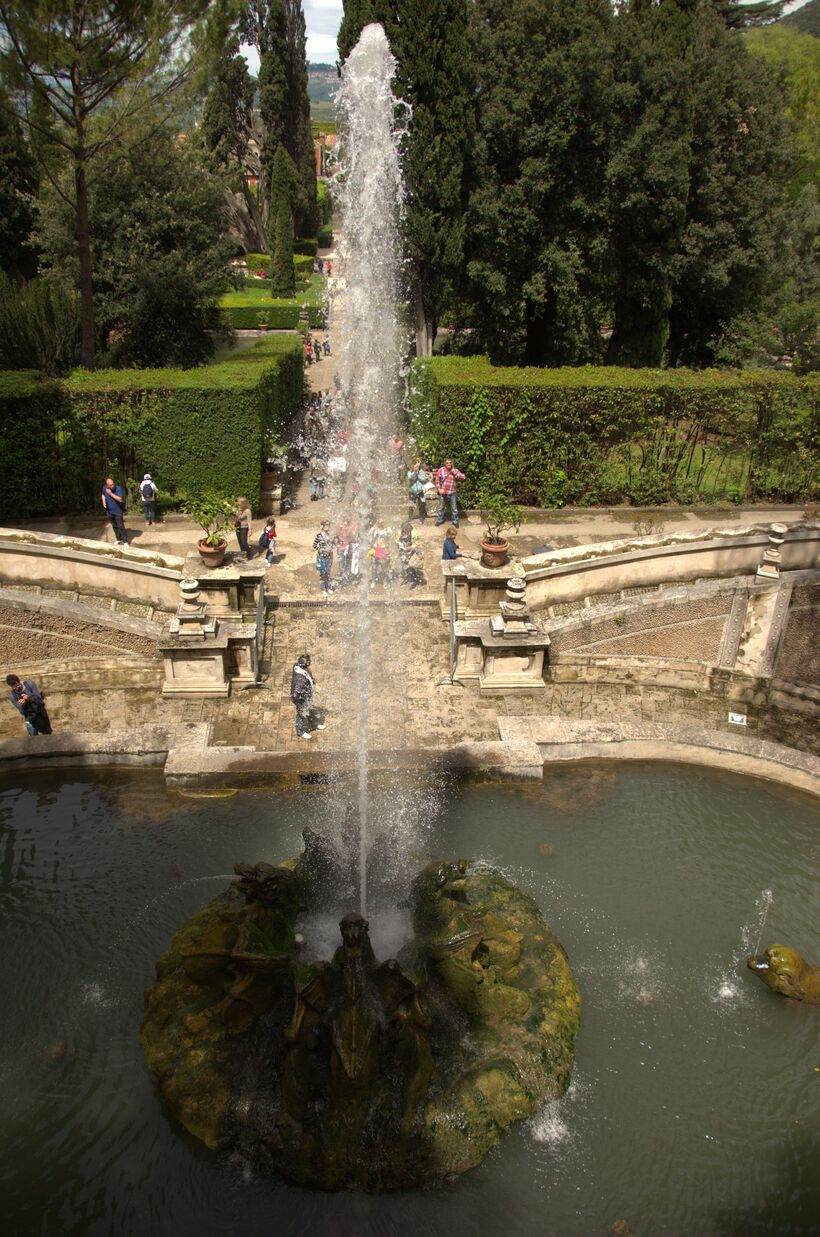
\includegraphics[height=\linewidth]{images/original/r002fc3e2t.jpeg}
    \caption{r002fc3e2t}
    \end{subfigure}\hfill%
    \begin{subfigure}[c]{.31\linewidth}\centering
    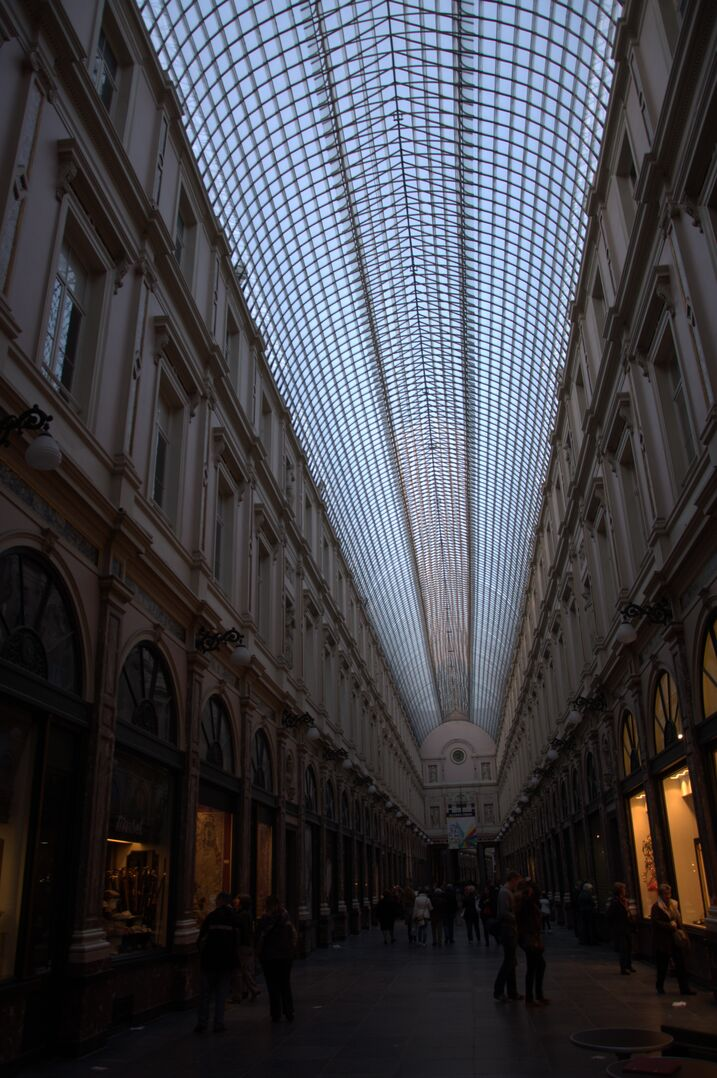
\includegraphics[height=\linewidth]{images/original/r1ead3024t.jpeg}
    \caption{r1ead3024t}
    \end{subfigure}\hfill%
    \begin{subfigure}[c]{.31\linewidth}\centering
    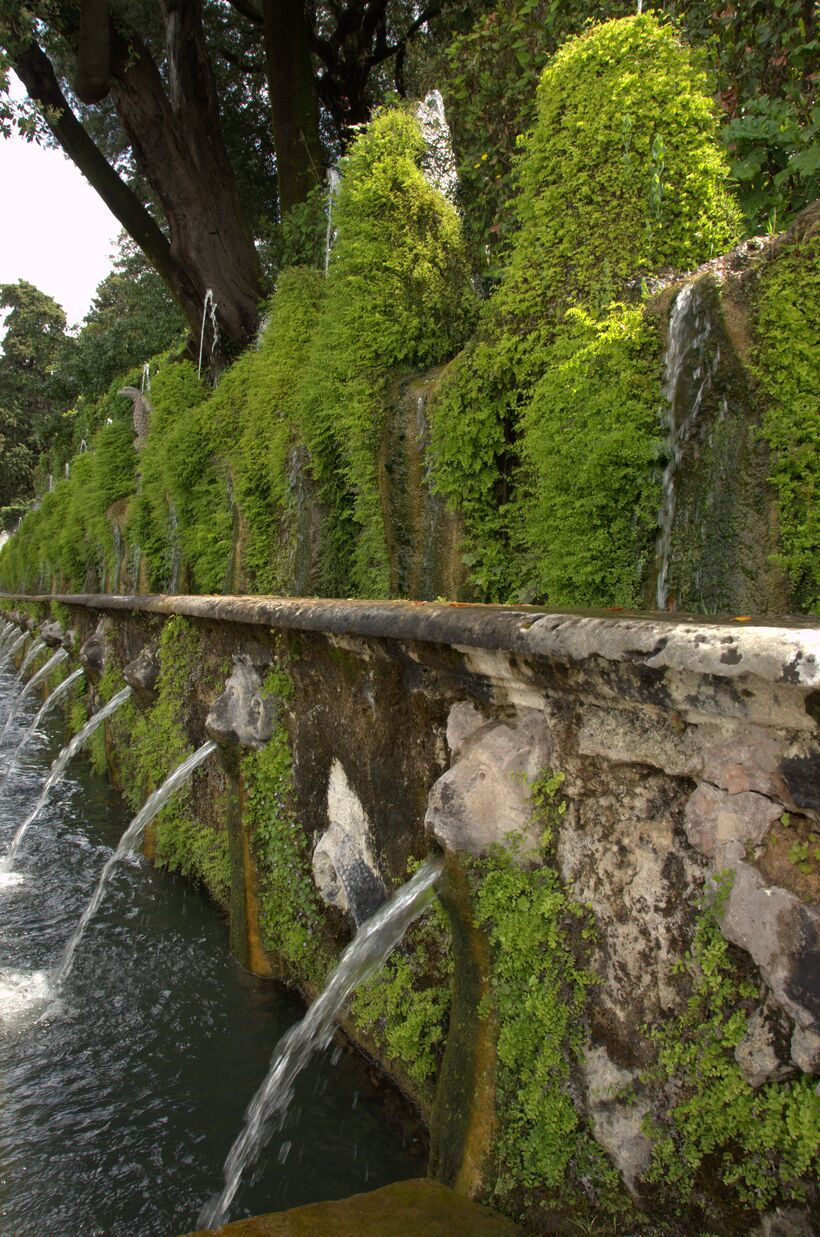
\includegraphics[height=\linewidth]{images/original/r1ceba29dt.jpeg}
    \caption{r1ceba29dt}
    \end{subfigure}%
    
    \begin{subfigure}[c]{.31\linewidth}\centering
    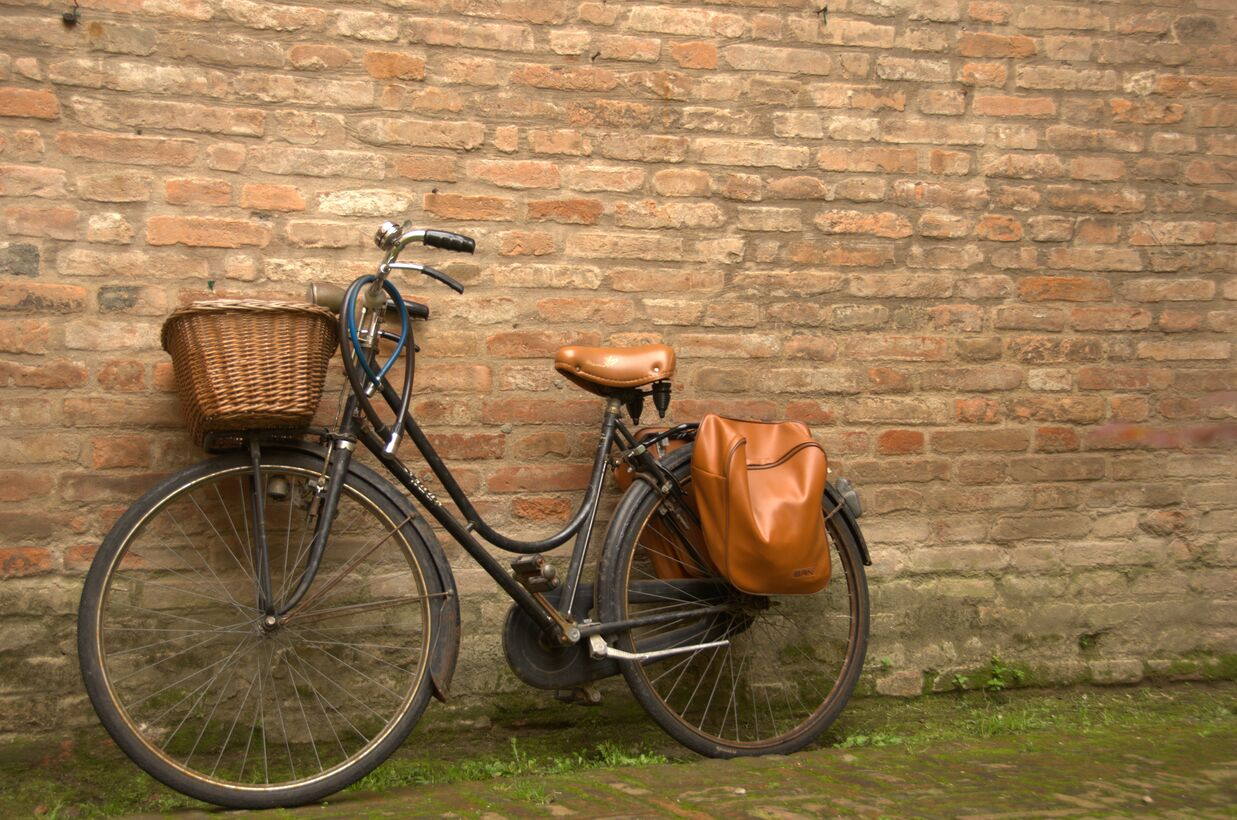
\includegraphics[width=\linewidth]{images/original/r0a2ff882t.jpeg}
    \caption{r0a2ff882t}
    \end{subfigure}\hfill%
    \begin{subfigure}[c]{.31\linewidth}\centering
    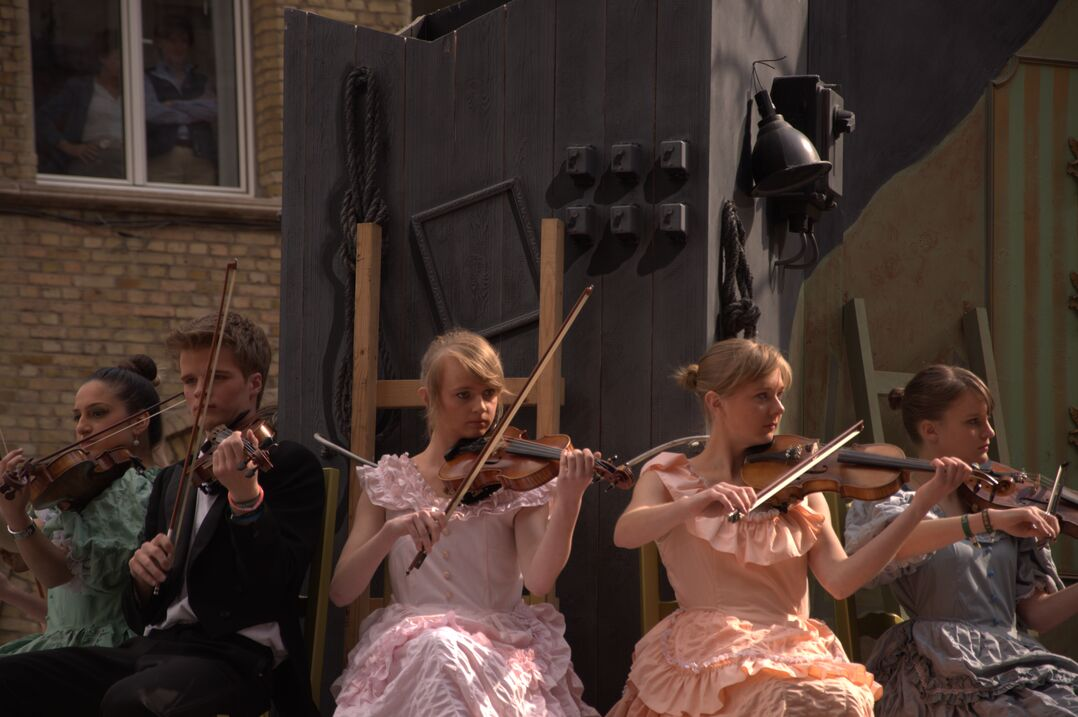
\includegraphics[width=\linewidth]{images/original/r0a808003t.jpeg}
    \caption{r0a808003t}
    \end{subfigure}\hfill%
    \begin{subfigure}[c]{.31\linewidth}\centering
    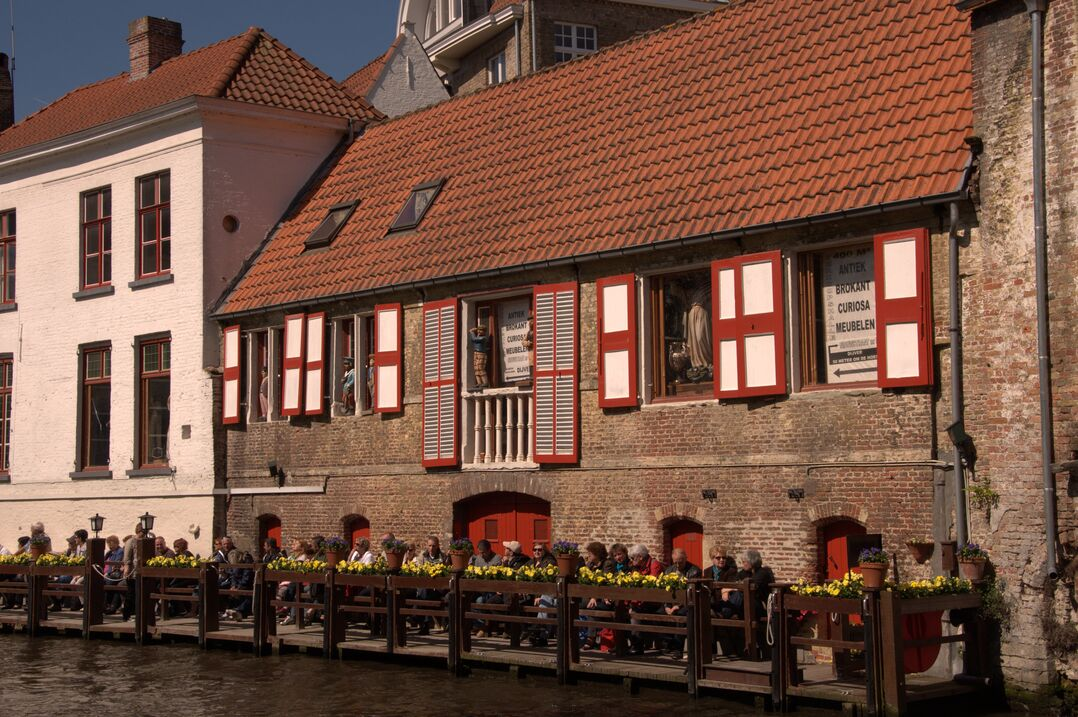
\includegraphics[width=\linewidth]{images/original/r0a966704t.jpeg}
    \caption{r0a966704t}
    \end{subfigure}
    
    \begin{subfigure}[c]{.31\linewidth}\centering
    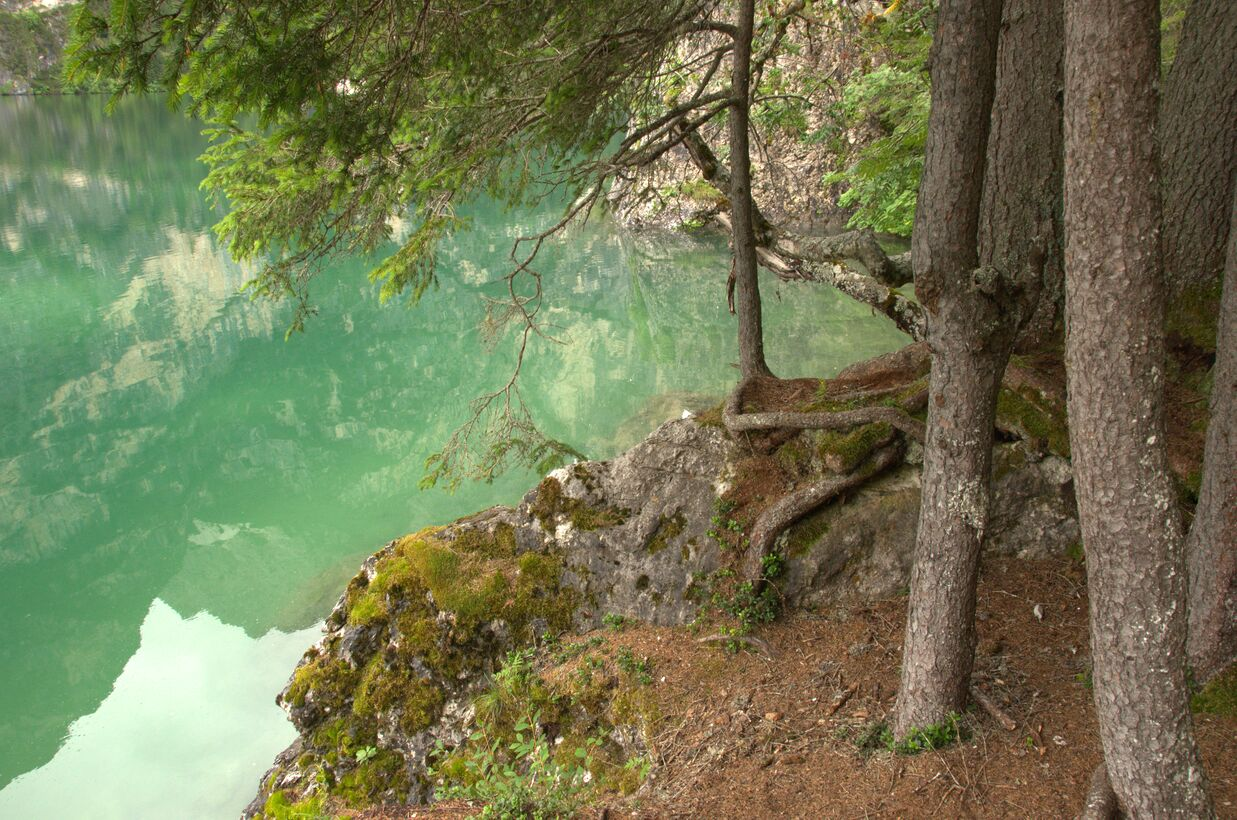
\includegraphics[width=\linewidth]{images/original/r0e04cc91t.jpeg}
    \caption{r0e04cc91t}
    \end{subfigure}\hfill%
    \begin{subfigure}[c]{.31\linewidth}\centering
    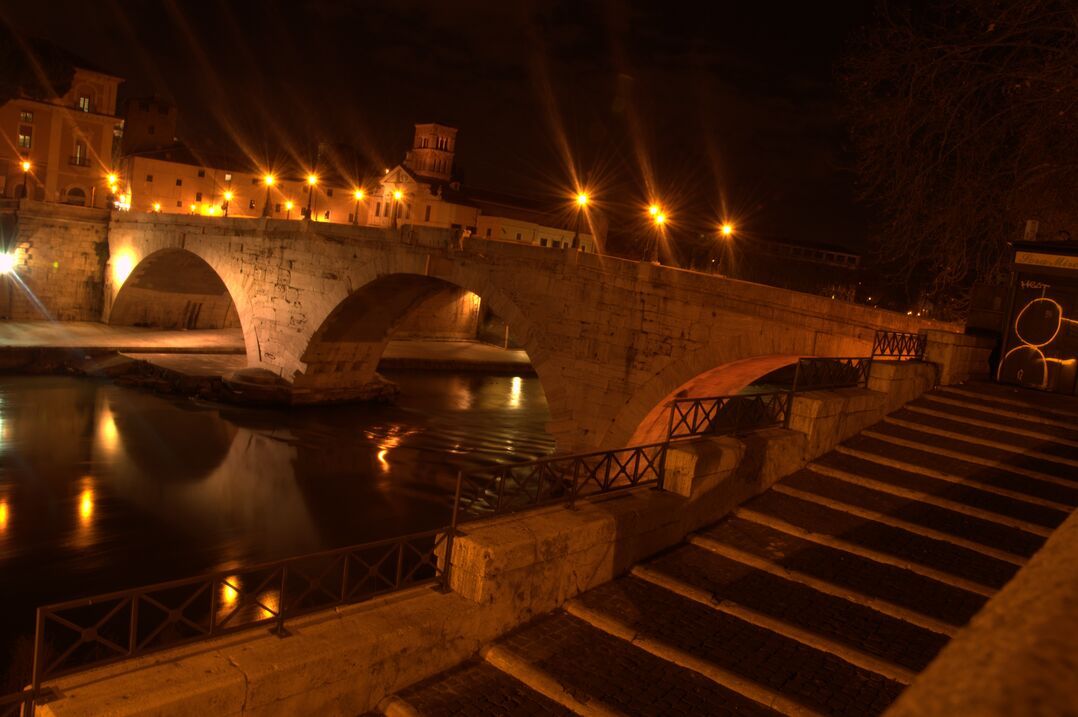
\includegraphics[width=\linewidth]{images/original/r0ea0825ft.jpeg}
    \caption{r0ea0825ft}
    \end{subfigure}\hfill%
    \begin{subfigure}[c]{.31\linewidth}\centering
    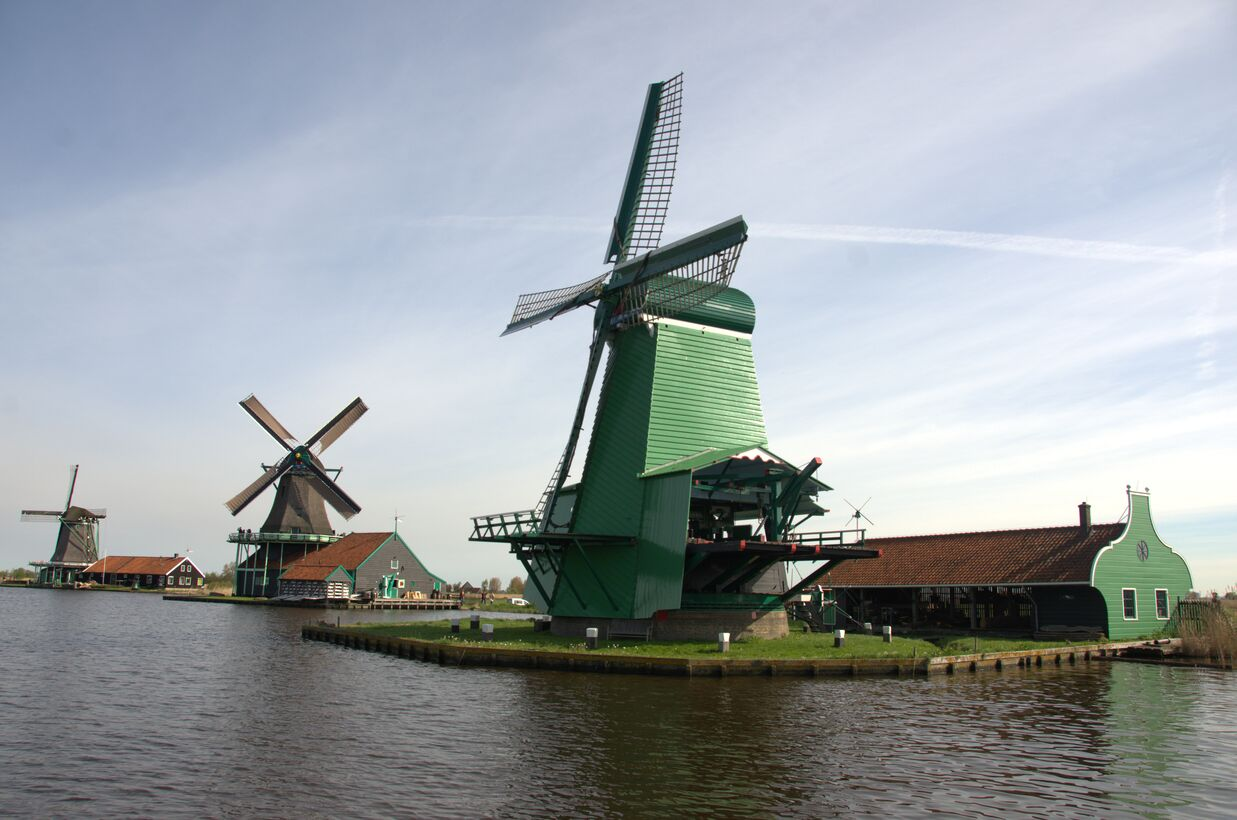
\includegraphics[width=\linewidth]{images/original/r1a0f5585t.jpeg}
    \caption{r1a0f5585t}
    \end{subfigure}
    
    \begin{subfigure}[c]{.31\linewidth}\centering
    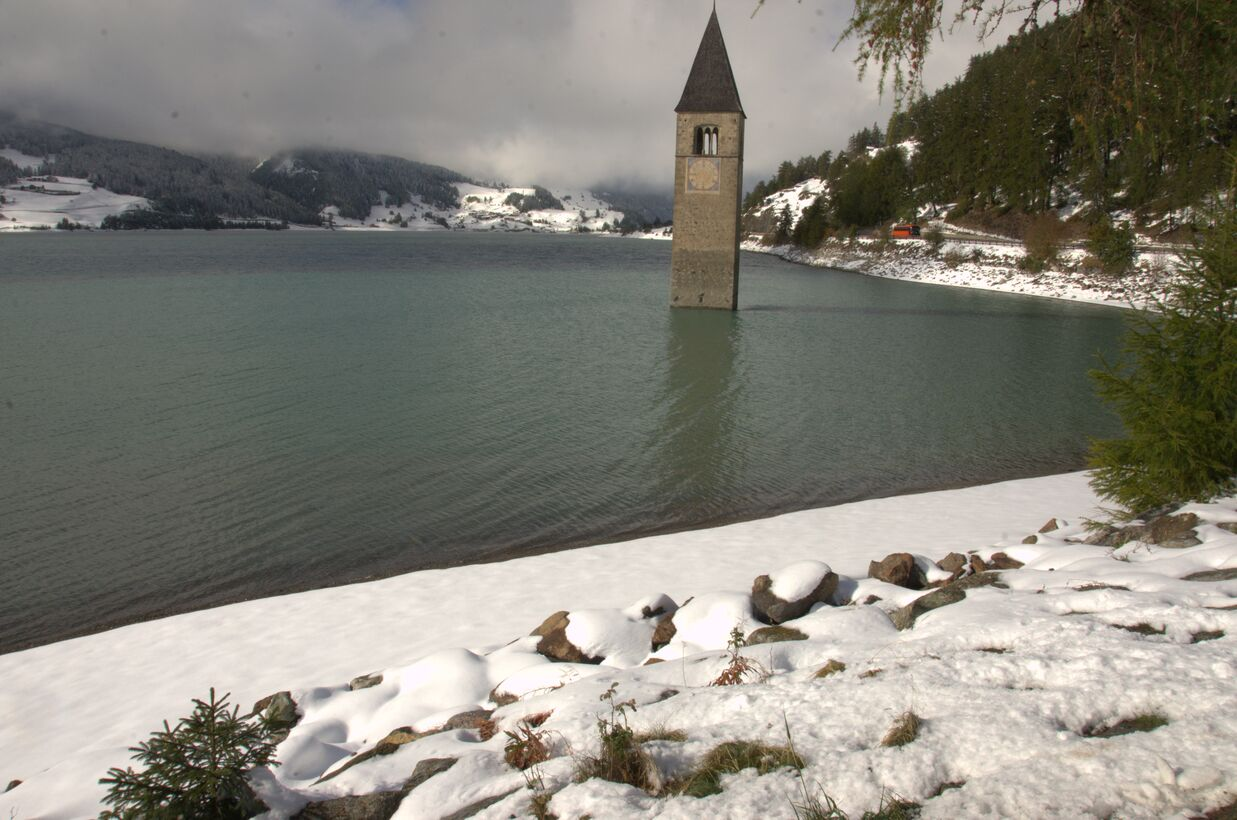
\includegraphics[width=\linewidth]{images/original/r1c9fdcf4t.jpeg}
    \caption{r1c9fdcf4t}
    \end{subfigure}\hfill%
    \begin{subfigure}[c]{.31\linewidth}\centering
    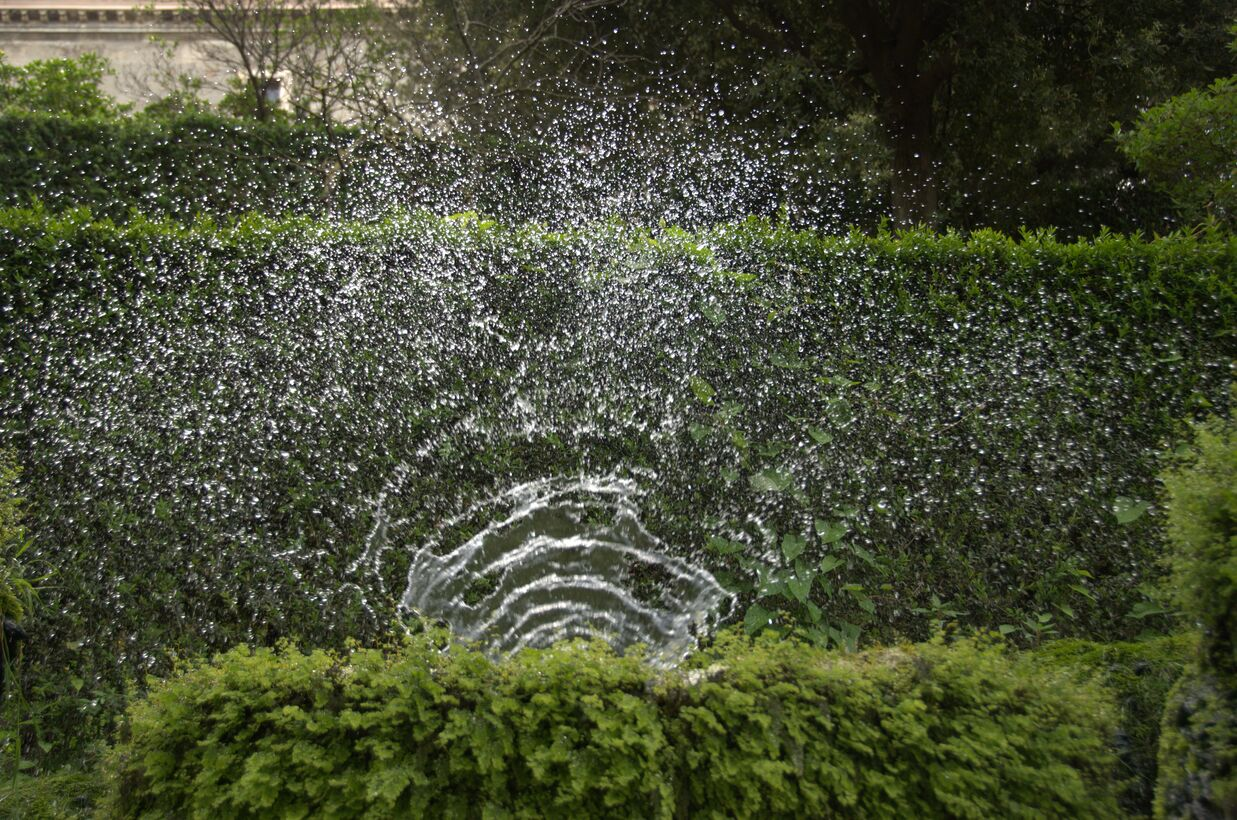
\includegraphics[width=\linewidth]{images/original/r06aa7dabt.jpeg}
    \caption{r06aa7dabt}
    \end{subfigure}\hfill%
    \begin{subfigure}[c]{.31\linewidth}\centering
    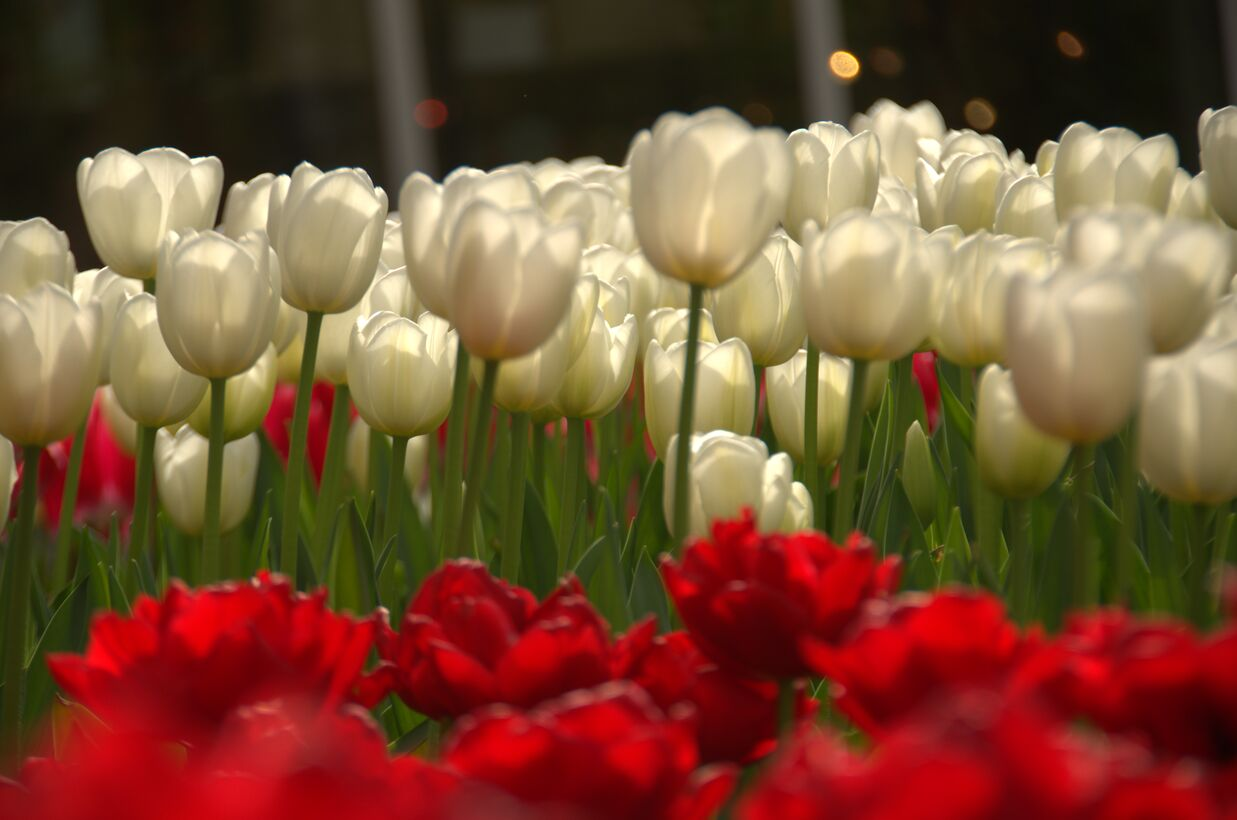
\includegraphics[width=\linewidth]{images/original/r07cfb432t.jpeg}
    \caption{r07cfb432t}
    \end{subfigure}
    
    \begin{subfigure}[c]{.31\linewidth}\centering
    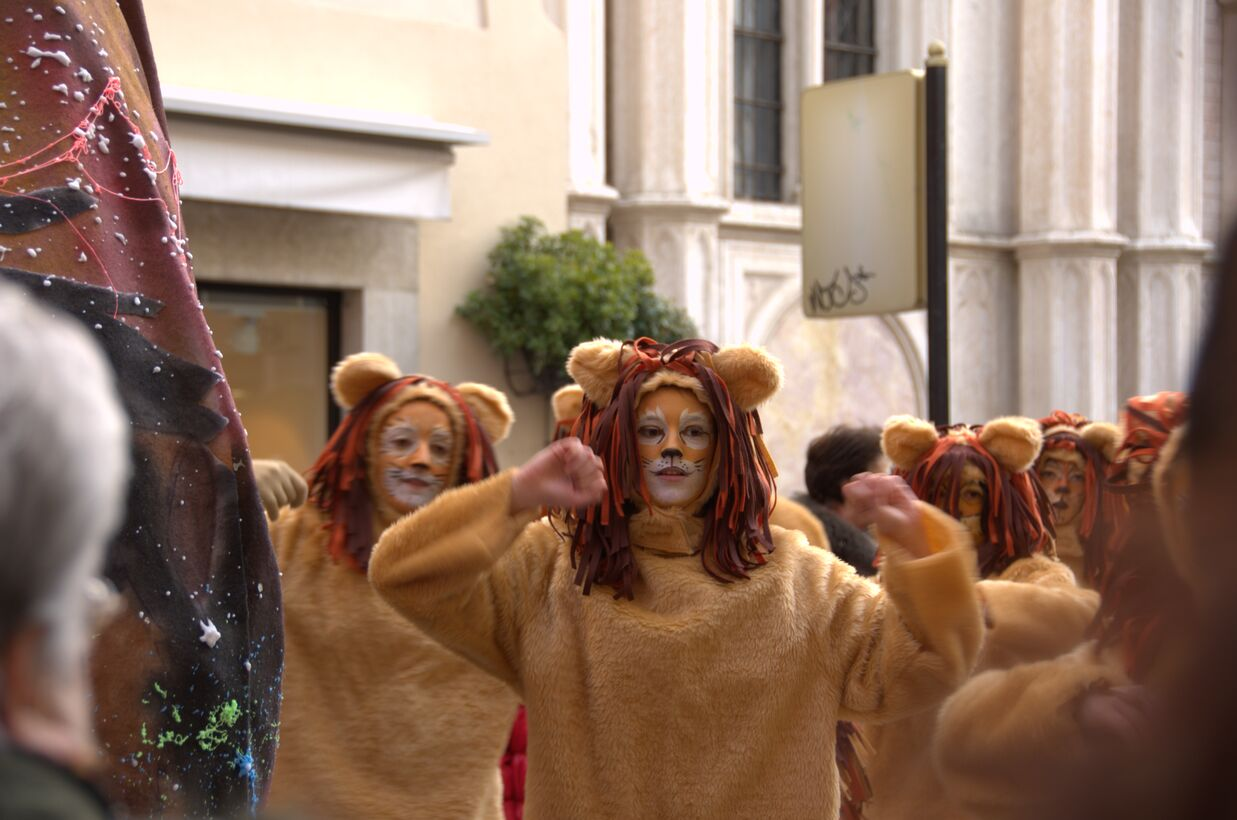
\includegraphics[width=\linewidth]{images/original/r07ffdc87t.jpeg}
    \caption{r07ffdc87t}
    \end{subfigure}\hfill%
    \begin{subfigure}[c]{.31\linewidth}\centering
    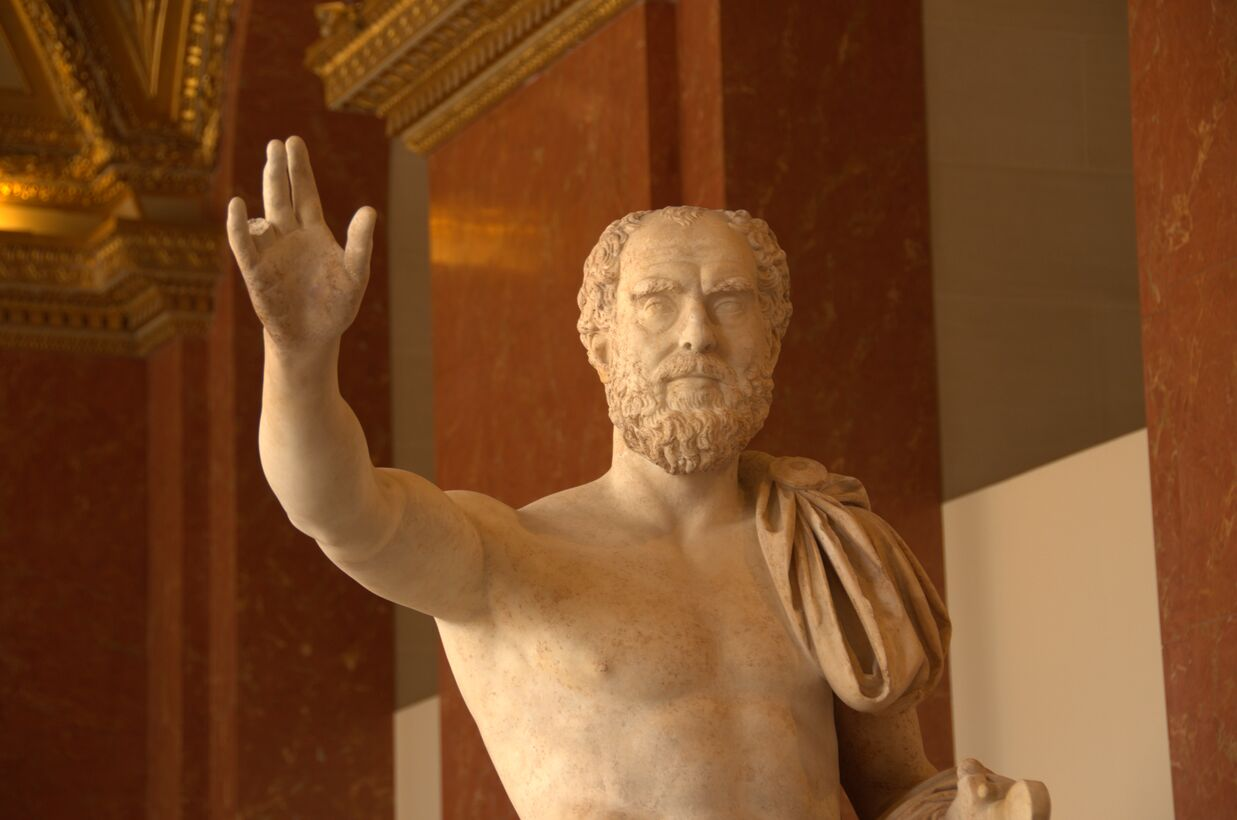
\includegraphics[width=\linewidth]{images/original/r16da5576t.jpeg}
    \caption{r16da5576t}
    \end{subfigure}\hfill%
    \begin{subfigure}[c]{.31\linewidth}\centering
    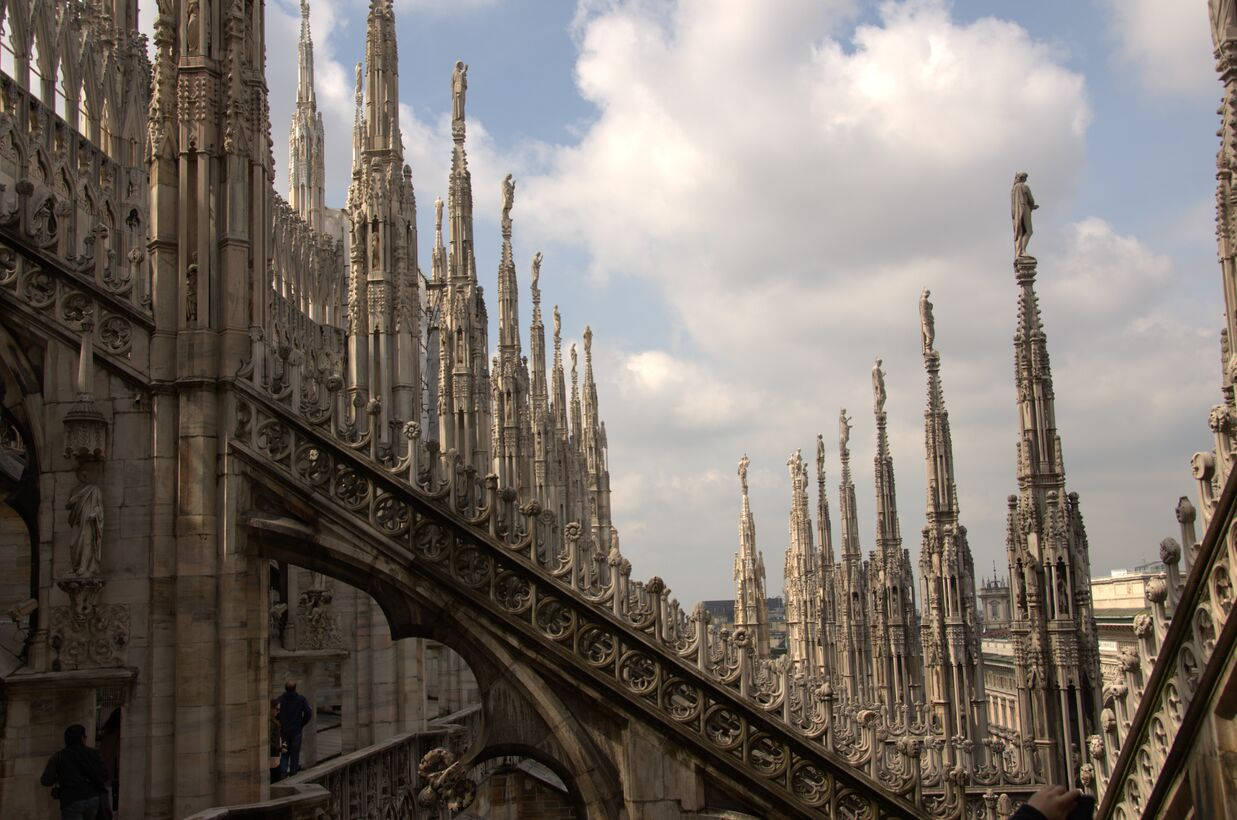
\includegraphics[width=\linewidth]{images/original/r191f3cdet.jpeg}
    \caption{r191f3cdet}
    \end{subfigure}
    
    \caption{Those 15 images from the Raise Dataset~\cite{raise} were used during our experiments.}
    \label{fig:15images}
\end{figure}

\subsection{CFA pattern detection}
\iffalse
\begin{table}[ht]
    \centering
    \begin{tabular}{lcc}
    \toprule
    Demosaicking & Diagonal & Full pattern\\
    \midrule
    AAHD & \color{c2}0/15 & \color{c2}0/15\\
    AHD & \color{c0}15/15 & \color{c0}15/15\\
    DCB & \color{c0}15/15 & \color{c0}15/15\\
    DHT & \color{c2}3/15 & \color{c2}3/15\\
    Bilinear & \color{c0}15/15 & \color{c0}15/15\\
    PPG & \color{c0}15/15 & \color{c3}13/15\\
    VNG & \color{c0}15/15 & \color{c3}14/15\\
    \bottomrule
    \end{tabular}
    \caption{Identification of the main diagonal and of the full pattern on the 15 images. The algorithm works very well when the demosaicking is done with AHD, DCB or Bilinear demosaicking, with a few errors on the full pattern against PPG- or VNG-demosaicked images. It fails to detect even the diagonal on AAHD- and DHT-demosaicked images}
    \label{tab:global}
\end{table}

\def\s{.12\linewidth}
\setlength{\tabcolsep}{0.2em}
\begin{figure}[ht]
        \centering
        \begin{tabular}{cccccccc}
                \multicolumn{8}{c}{
                        \begin{tabular}{cl}
                                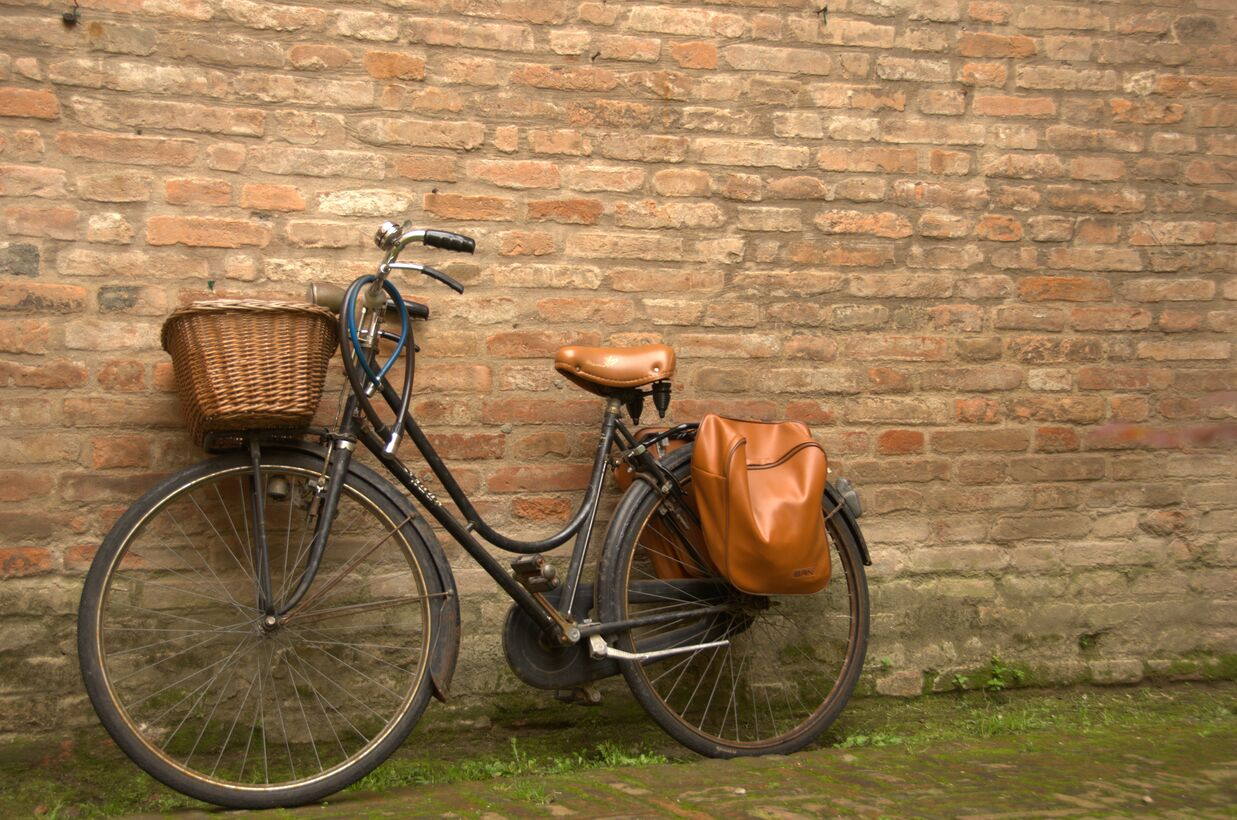
\includegraphics[width=.6\linewidth]{images/original/r0a2ff882t.jpeg}&
                                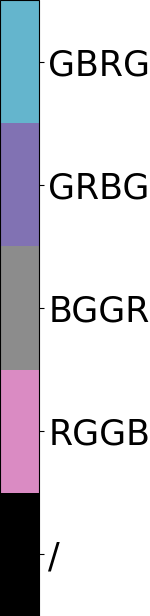
\includegraphics[height=150pt]{images/cb.png}\\
                                Original image (r0a2ff882t), in \textsc{rggb} pattern&
                        \end{tabular}
                }\\                                
                & AAHD & AHD & DCB & DHT & Bilinear & PPG & VNG\\
                \midrule
                \raisebox{5pt}{\rotatebox{90}{\tiny Original}} & 
                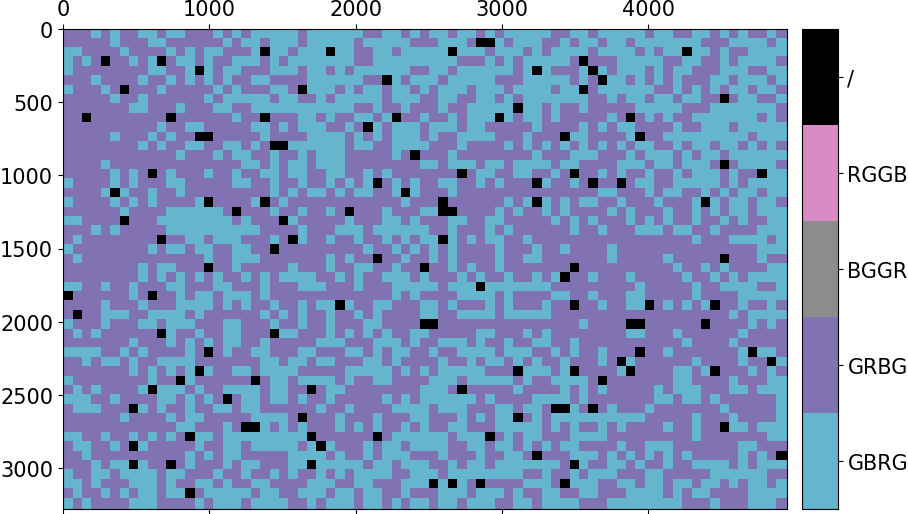
\includegraphics[width=\s]{images/bike/AAHD/iso_64_grids.png} &
                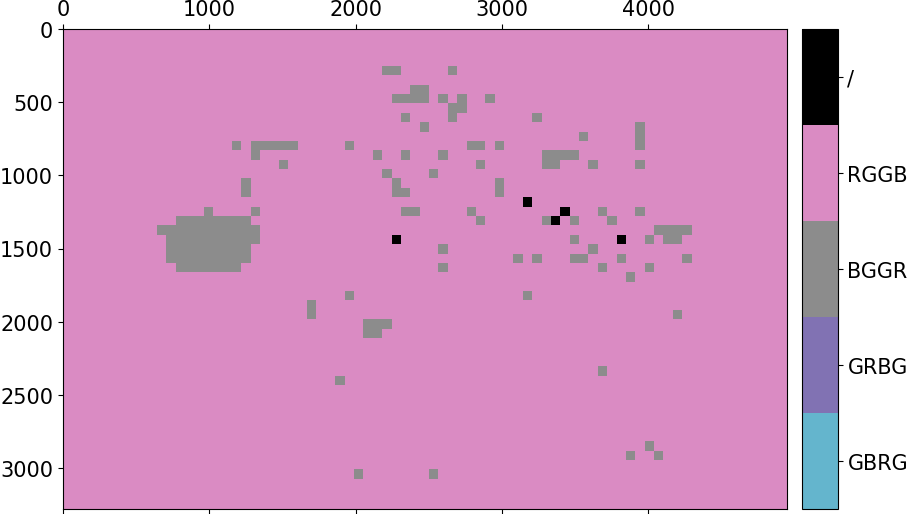
\includegraphics[width=\s]{images/bike/AHD/iso_64_grids.png} &
                
\includegraphics[width=\s]{images/bike/DCB/iso_64_grids.png} &
                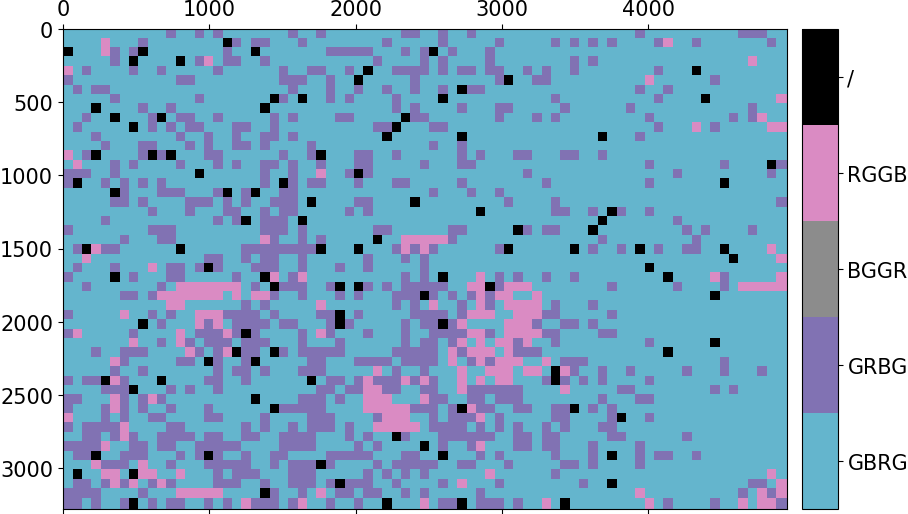
\includegraphics[width=\s]{images/bike/DHT/iso_64_grids.png} &
                
\includegraphics[width=\s]{images/bike/LINEAR/iso_64_grids.png} &
                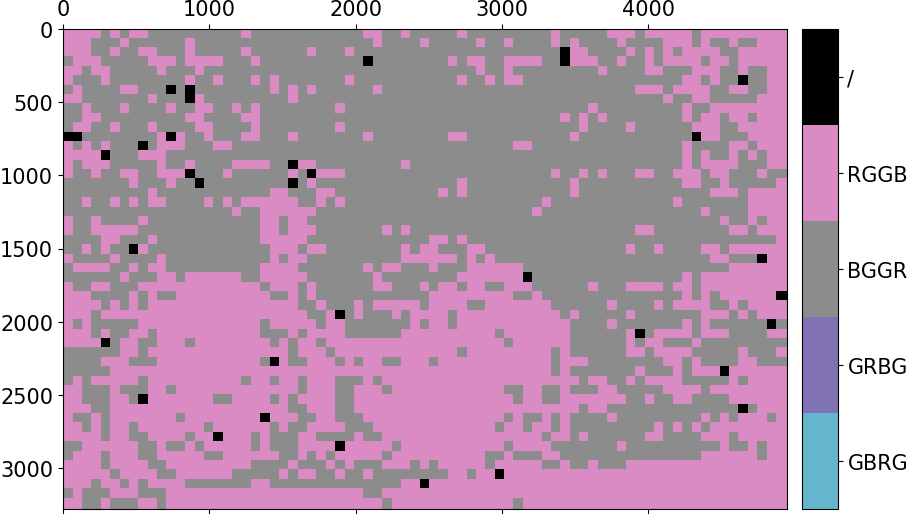
\includegraphics[width=\s]{images/bike/PPG/iso_64_grids.png} &
                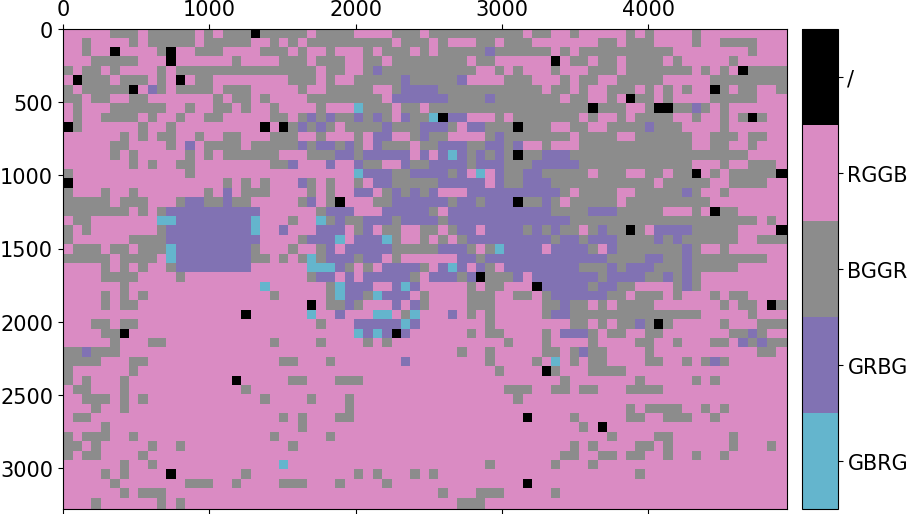
\includegraphics[width=\s]{images/bike/VNG/iso_64_grids.png} \\
                \rotatebox{90}{\tiny Bidirectional} & 
                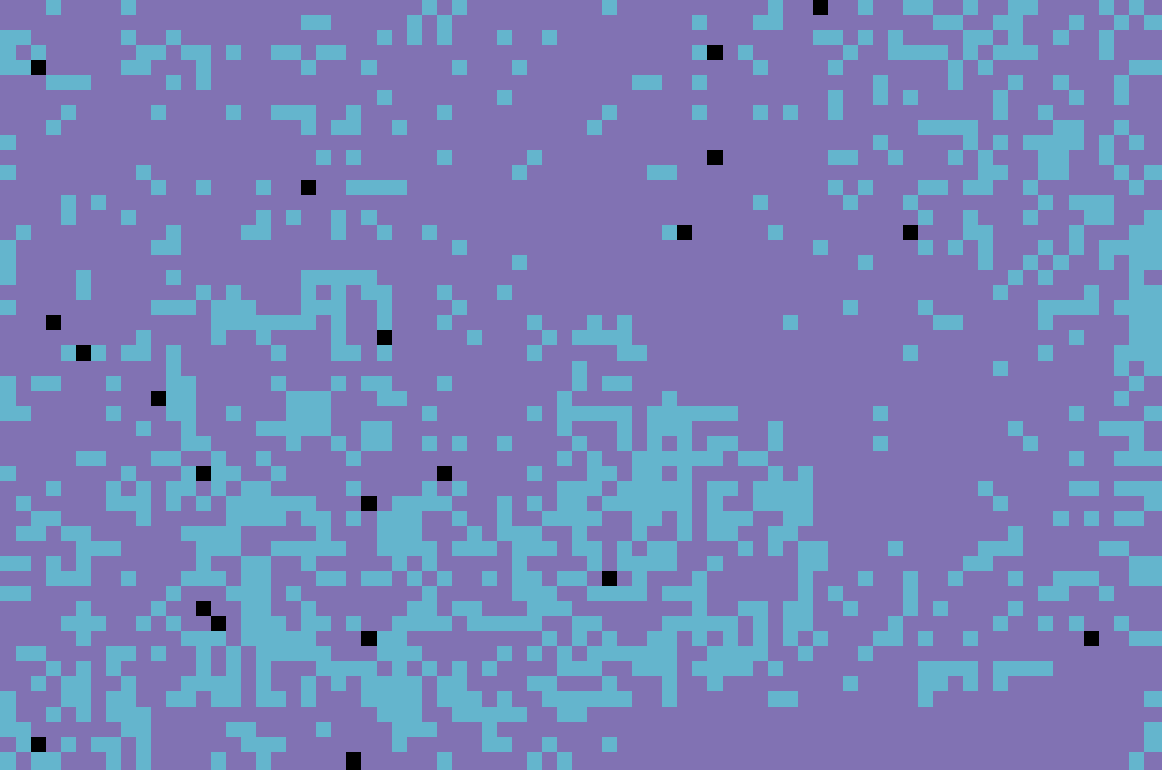
\includegraphics[width=\s]{images/bike/AAHD/bid_64_grids.png} &
                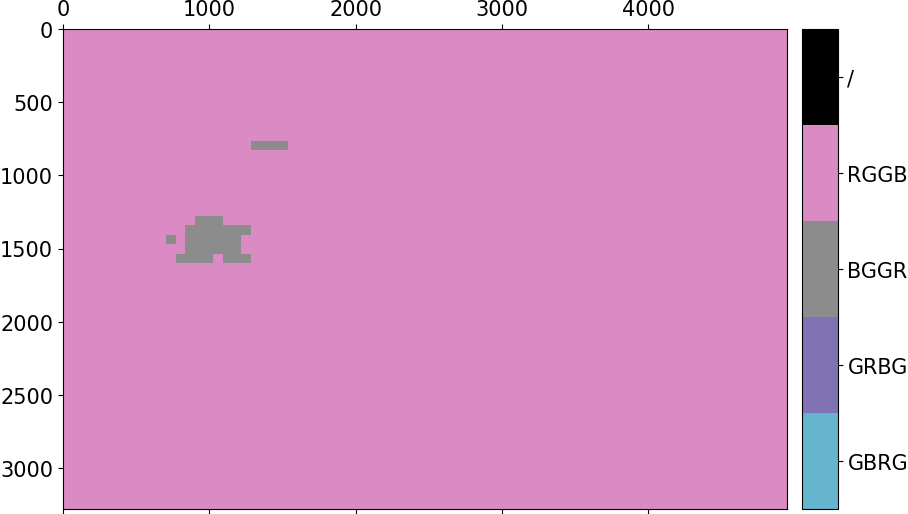
\includegraphics[width=\s]{images/bike/AHD/bid_64_grids.png} &
                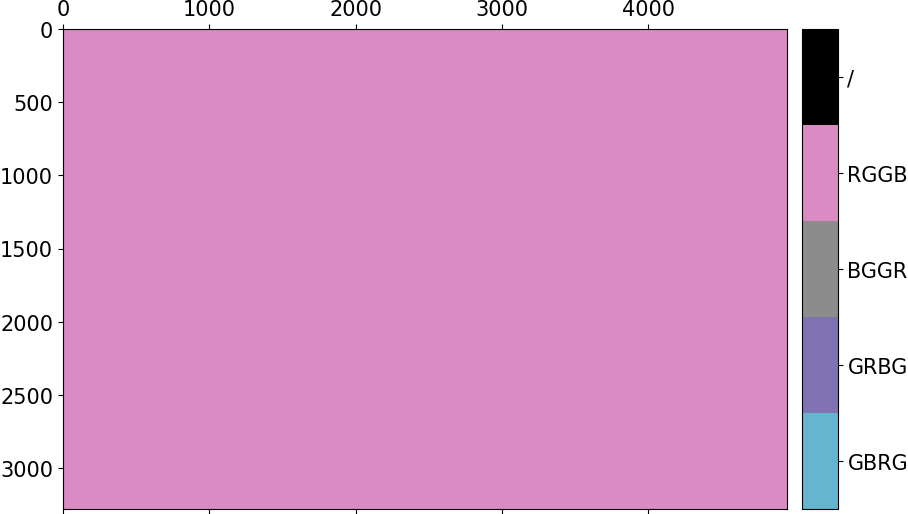
\includegraphics[width=\s]{images/bike/DCB/bid_64_grids.png} &
                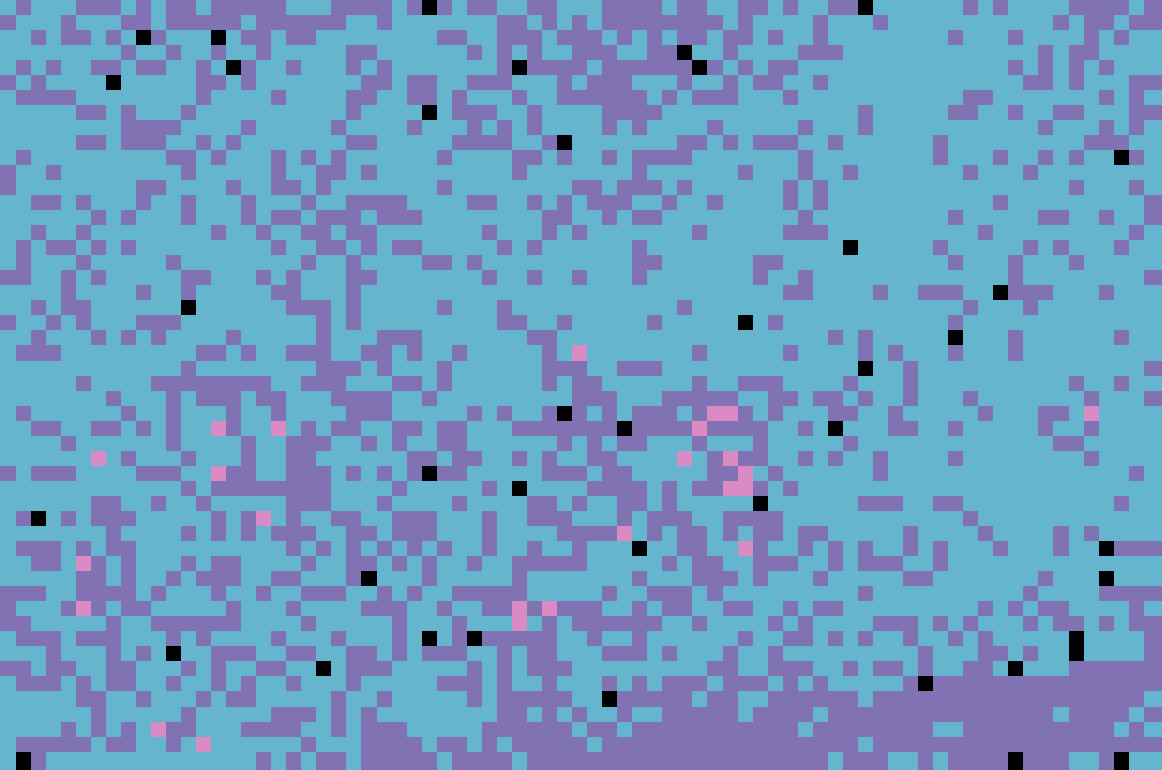
\includegraphics[width=\s]{images/bike/DHT/bid_64_grids.png} &
                
\includegraphics[width=\s]{images/bike/LINEAR/bid_64_grids.png} &
                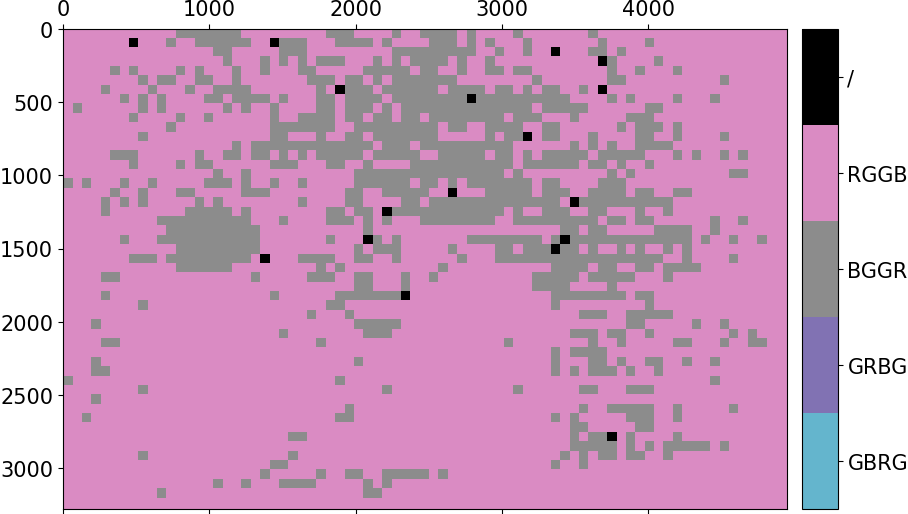
\includegraphics[width=\s]{images/bike/PPG/bid_64_grids.png} &
                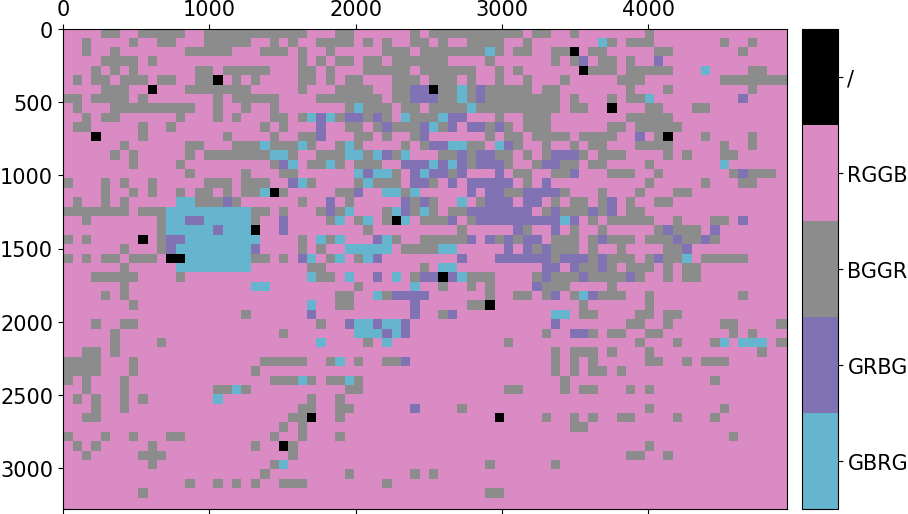
\includegraphics[width=\s]{images/bike/VNG/bid_64_grids.png}\\
                \bottomrule
        \end{tabular}
\caption{Results of the method on 64×64 windows, both with the original isotropic intermediate value mask and the proposed bidirectional one, on one image with the 7 different demosaicing algorithms. Both method work perfectly on the DCB- and Bilinear-demosaiced images. With the AHD, PPG and VNG methods, both methods have trouble discerning between the two patterns sharing the same diagonal, but the bidirectional detection makes fewer mistakes. Textured regions such as the basket can create a localized shift in the detected mosaic, which could be interpretated as a forgery.
With the AAHD and DHT algorithm, the method consistently detects the wrong diagonal.}
\label{fig:bike}
\end{figure}



\begin{figure}[ht]
\centering
\begin{subfigure}[t]{.5\linewidth}
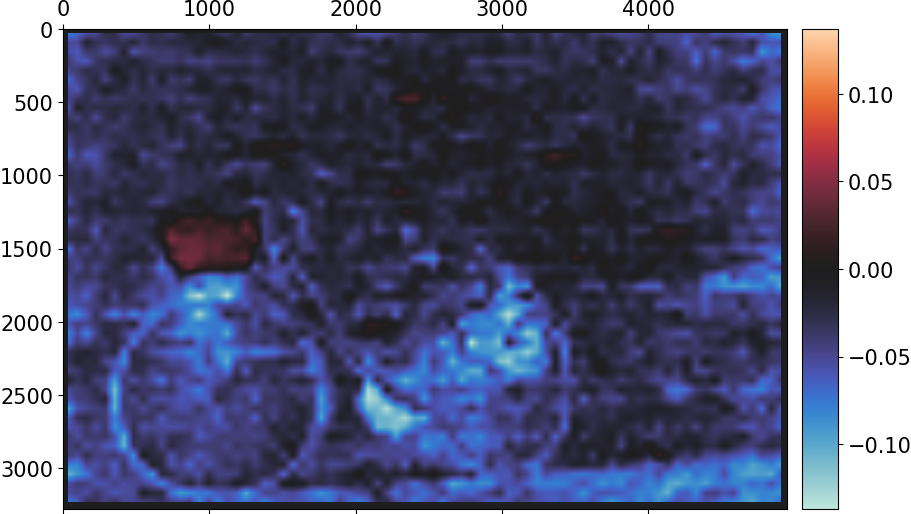
\includegraphics[width=\linewidth]{images/bike/ahd_iso_64_diff_rggb_bggr.png}
\caption{Isotropic}
\end{subfigure}%
\begin{subfigure}[t]{.5\linewidth}
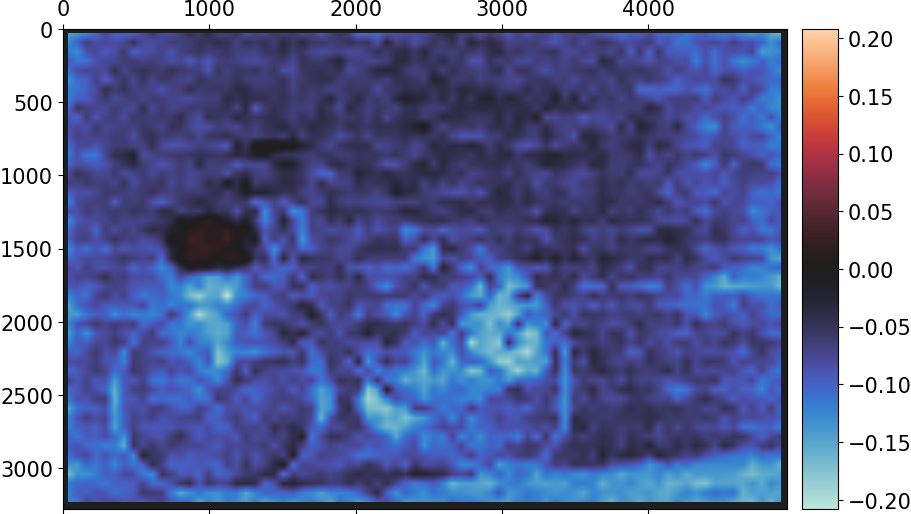
\includegraphics[width=\linewidth]{images/bike/ahd_bid_64_diff_rggb_bggr.png}
\caption{Bidirectional}
\end{subfigure}%
\caption{This figure shows, on the AHD-demosaiced bicycle image, the difference of counts of intermediate values corresponding to the \textsc{rggb} and \textsc{bggr} patterns, on the red and blue channels. This count is what is used by the algorithm to decide on a grid. A negative difference corresponds to the correct \textsc{rggb} pattern, a positive difference to the incorrect \textsc{bggr} pattern. The difference is normalized by dividing it by the size of the block ($64\times64$). The textures in the basket area leads to a locally consistent shift in the position of the intermediate values. The error is slightly less prominent when a bidirectional mask is used, but is still consistently in favour of the wrong grid.}
\end{figure}

\begin{figure}[ht]
        \centering
        \begin{subfigure}[t]{\linewidth}
        \begin{tabular}{ccccccccc}
                \multicolumn{9}{c}{
                        \begin{tabular}{cl}
                                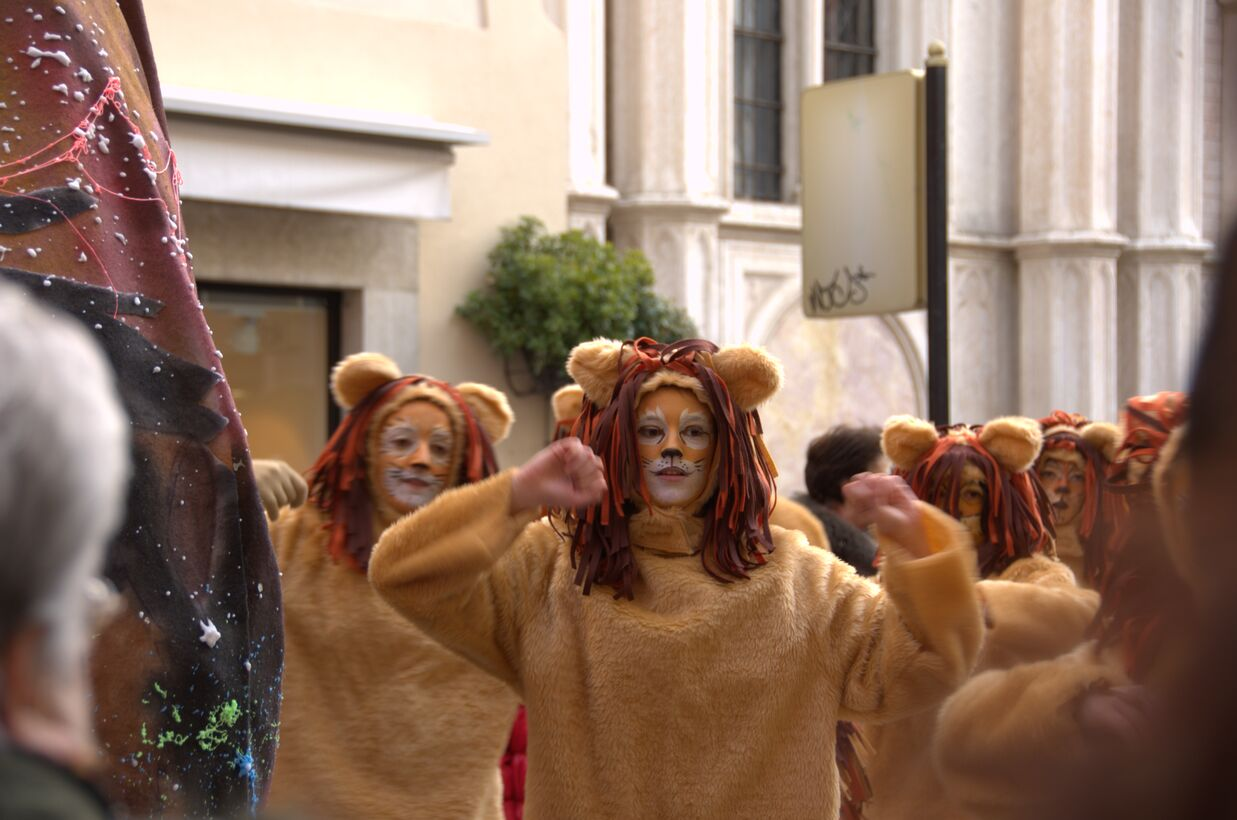
\includegraphics[height=150pt]{images/original/r07ffdc87t.jpeg}&
                                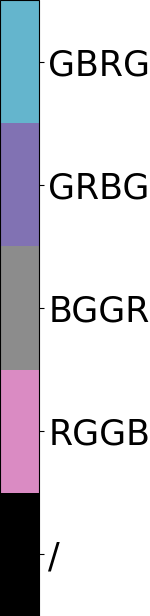
\includegraphics[height=150pt]{images/cb.png}
                        \end{tabular}
                }\\                                
                && AAHD & AHD & DCB & DHT & Bilinear & PPG & VNG\\
                \midrule
                \multirow{2}{*}[1.3em]{{\rotatebox[origin=c]{90}{Uncompressed}}}&
                \raisebox{5pt}{\rotatebox{90}{\tiny Original}} & 
                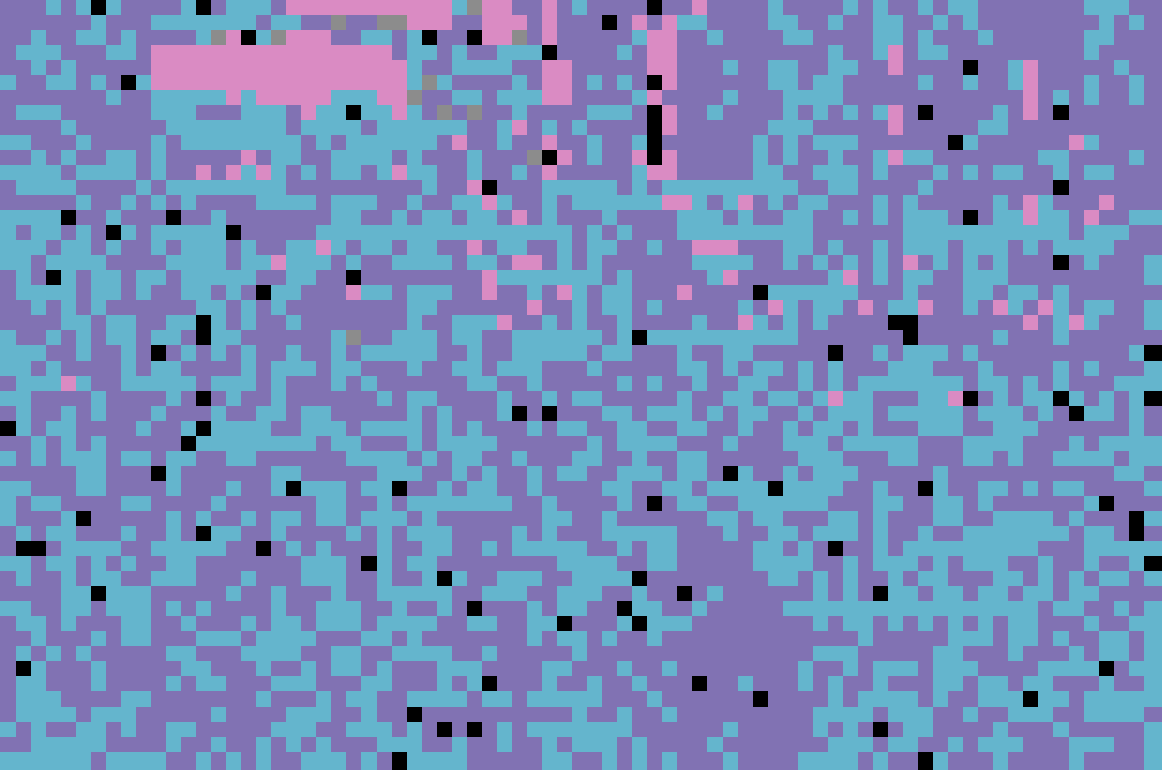
\includegraphics[width=\s]{images/carnival/AAHD/iso_64_grids.png}&
                
\includegraphics[width=\s]{images/carnival/AHD/iso_64_grids.png}&
                
\includegraphics[width=\s]{images/carnival/DCB/iso_64_grids.png}&
                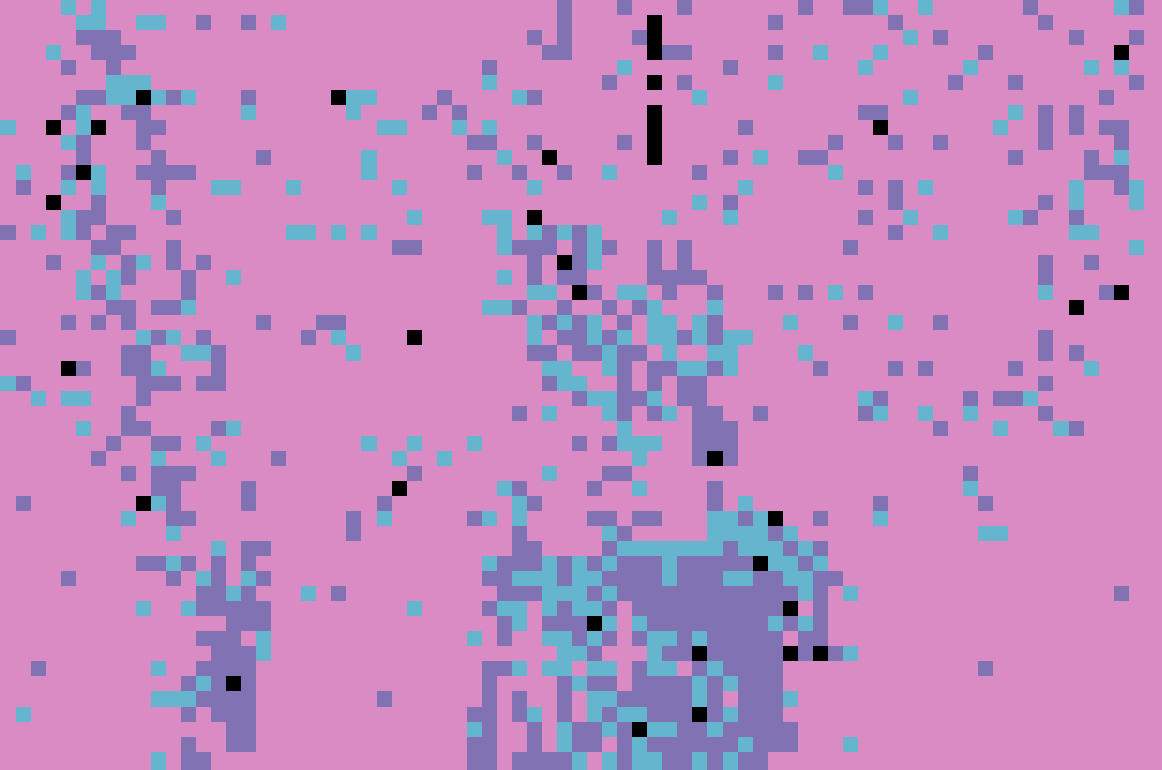
\includegraphics[width=\s]{images/carnival/DHT/iso_64_grids.png}&
                
\includegraphics[width=\s]{images/carnival/LINEAR/iso_64_grids.png}&
                
\includegraphics[width=\s]{images/carnival/PPG/iso_64_grids.png}&
                
\includegraphics[width=\s]{images/carnival/VNG/iso_64_grids.png}\\
                &\rotatebox{90}{\tiny Bidirectional}&
                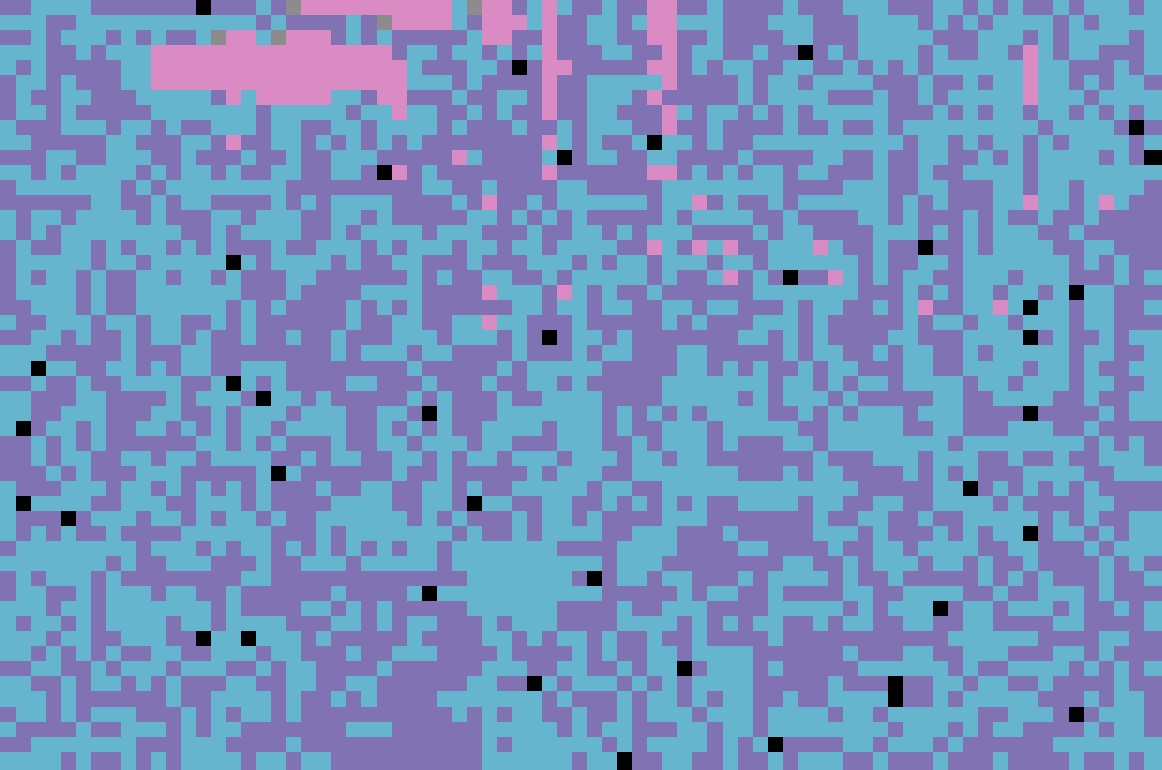
\includegraphics[width=\s]{images/carnival/AAHD/bid_64_grids.png}&
                
\includegraphics[width=\s]{images/carnival/AHD/bid_64_grids.png}&
                
\includegraphics[width=\s]{images/carnival/DCB/bid_64_grids.png}&
                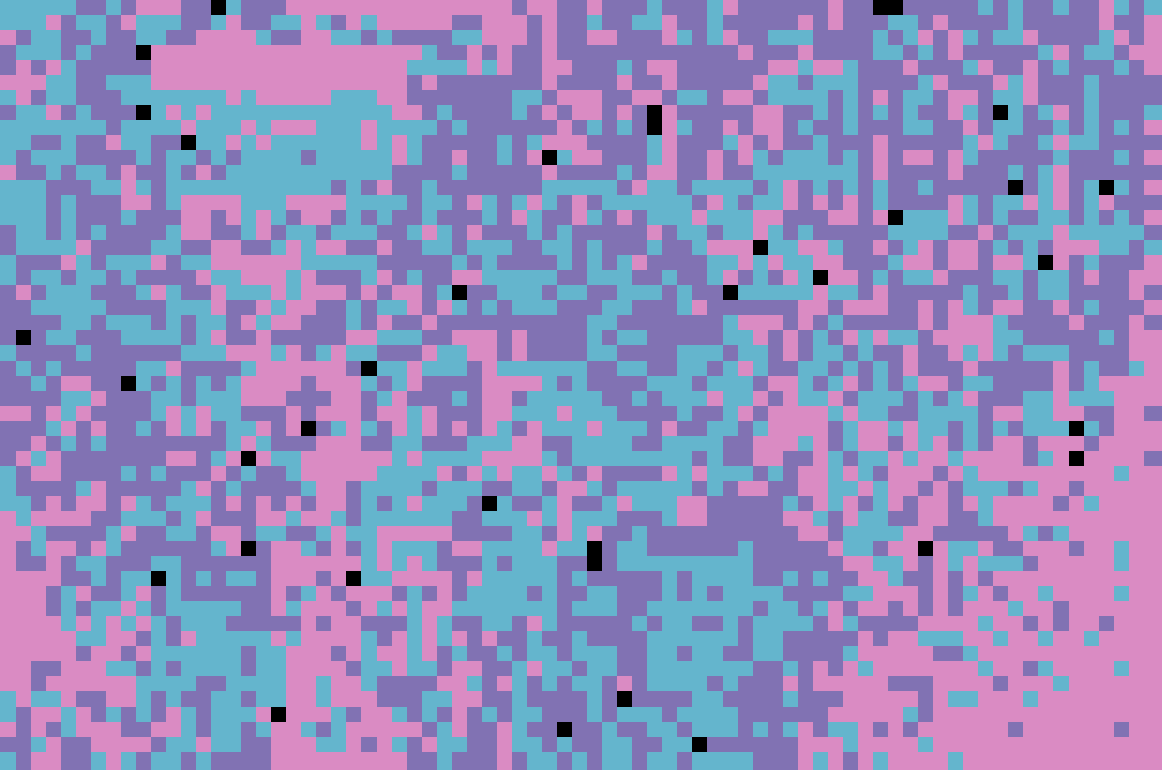
\includegraphics[width=\s]{images/carnival/DHT/bid_64_grids.png}&
                
\includegraphics[width=\s]{images/carnival/LINEAR/bid_64_grids.png}&
                
\includegraphics[width=\s]{images/carnival/PPG/bid_64_grids.png}&
                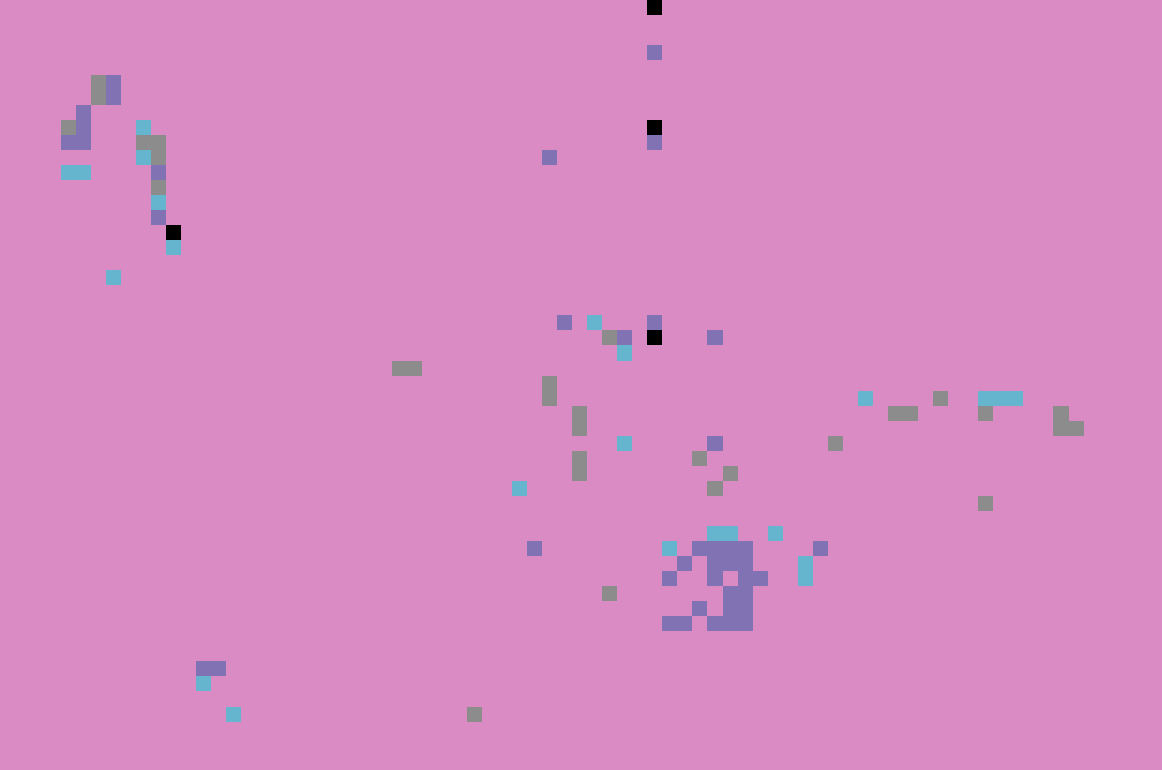
\includegraphics[width=\s]{images/carnival/VNG/bid_64_grids.png}\\
                \cmidrule{1-2}
                \multirow{2}{*}[.5em]{{\rotatebox[origin=c]{90}{JPEG 100}}}&
                \raisebox{5pt}{\rotatebox{90}{\tiny Original}} & 
                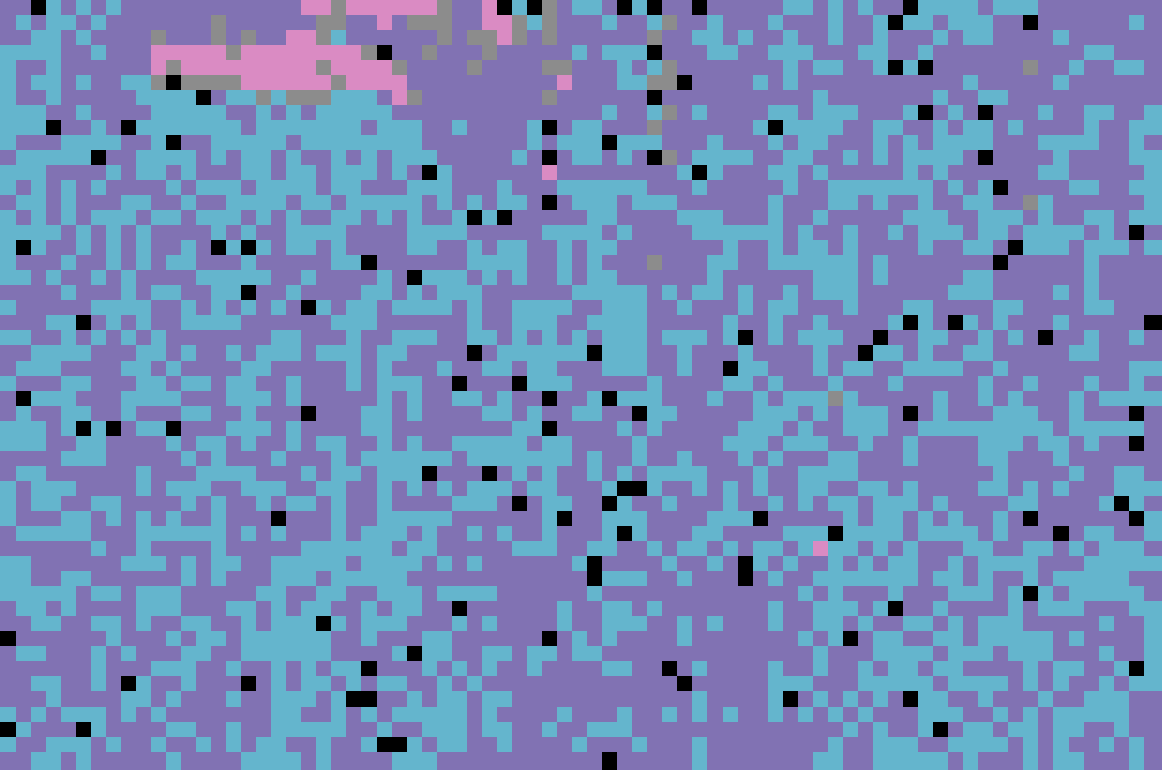
\includegraphics[width=\s]{images/carnival/AAHD/iso_j100_64_grids.png}&
                \includegraphics[width=\s]{images/carnival/AHD/iso_j100_64_grids.png}&
                \includegraphics[width=\s]{images/carnival/DCB/iso_j100_64_grids.png}&
                \includegraphics[width=\s]{images/carnival/DHT/iso_j100_64_grids.png}&
                \includegraphics[width=\s]{images/carnival/LINEAR/iso_j100_64_grids.png}&
                \includegraphics[width=\s]{images/carnival/PPG/iso_j100_64_grids.png}&
                \includegraphics[width=\s]{images/carnival/VNG/iso_j100_64_grids.png}\\
                &\rotatebox{90}{\tiny Bidirectional}&
                \includegraphics[width=\s]{images/carnival/AAHD/bid_j100_64_grids.png}&
                \includegraphics[width=\s]{images/carnival/AHD/bid_j100_64_grids.png}&
                \includegraphics[width=\s]{images/carnival/DCB/bid_j100_64_grids.png}&
                \includegraphics[width=\s]{images/carnival/DHT/bid_j100_64_grids.png}&
                \includegraphics[width=\s]{images/carnival/LINEAR/bid_j100_64_grids.png}&
                \includegraphics[width=\s]{images/carnival/PPG/bid_j100_64_grids.png}&
                \includegraphics[width=\s]{images/carnival/VNG/bid_j100_64_grids.png}\\
                \cmidrule{1-2}
                \multirow{2}{*}[.5em]{{\rotatebox[origin=c]{90}{JPEG 98}}}&
                \raisebox{5pt}{\rotatebox{90}{\tiny Original}} & 
                \includegraphics[width=\s]{images/carnival/AAHD/iso_j98_64_grids.png}&
                \includegraphics[width=\s]{images/carnival/AHD/iso_j98_64_grids.png}&
                \includegraphics[width=\s]{images/carnival/DCB/iso_j98_64_grids.png}&
                \includegraphics[width=\s]{images/carnival/DHT/iso_j98_64_grids.png}&
                \includegraphics[width=\s]{images/carnival/LINEAR/iso_j98_64_grids.png}&
                \includegraphics[width=\s]{images/carnival/PPG/iso_j98_64_grids.png}&
                \includegraphics[width=\s]{images/carnival/VNG/iso_j98_64_grids.png}\\
                &\rotatebox{90}{\tiny Bidirectional}&
                \includegraphics[width=\s]{images/carnival/AAHD/bid_j98_64_grids.png}&
                \includegraphics[width=\s]{images/carnival/AHD/bid_j98_64_grids.png}&
                \includegraphics[width=\s]{images/carnival/DCB/bid_j98_64_grids.png}&
                \includegraphics[width=\s]{images/carnival/DHT/bid_j98_64_grids.png}&
                \includegraphics[width=\s]{images/carnival/LINEAR/bid_j98_64_grids.png}&
                \includegraphics[width=\s]{images/carnival/PPG/bid_j98_64_grids.png}&
                \includegraphics[width=\s]{images/carnival/VNG/bid_j98_64_grids.png}\\
                \cmidrule{1-2}
                \multirow{2}{*}[.5em]{{\rotatebox[origin=c]{90}{JPEG 95}}}&
                \raisebox{5pt}{\rotatebox{90}{\tiny Original}} & 
                \includegraphics[width=\s]{images/carnival/AAHD/iso_j95_64_grids.png}&
                \includegraphics[width=\s]{images/carnival/AHD/iso_j95_64_grids.png}&
                \includegraphics[width=\s]{images/carnival/DCB/iso_j95_64_grids.png}&
                \includegraphics[width=\s]{images/carnival/DHT/iso_j95_64_grids.png}&
                \includegraphics[width=\s]{images/carnival/LINEAR/iso_j95_64_grids.png}&
                \includegraphics[width=\s]{images/carnival/PPG/iso_j95_64_grids.png}&
                \includegraphics[width=\s]{images/carnival/VNG/iso_j95_64_grids.png}\\
                &\rotatebox{90}{\tiny Bidirectional}&
                \includegraphics[width=\s]{images/carnival/AAHD/bid_j95_64_grids.png}&
                \includegraphics[width=\s]{images/carnival/AHD/bid_j95_64_grids.png}&
                \includegraphics[width=\s]{images/carnival/DCB/bid_j95_64_grids.png}&
                \includegraphics[width=\s]{images/carnival/DHT/bid_j95_64_grids.png}&
                \includegraphics[width=\s]{images/carnival/LINEAR/bid_j95_64_grids.png}&
                \includegraphics[width=\s]{images/carnival/PPG/bid_j95_64_grids.png}&
                \includegraphics[width=\s]{images/carnival/VNG/bid_j95_64_grids.png}\\
                \bottomrule
        \end{tabular}
        \caption{Image r07ffdc87t, in \textsc{rggb} pattern}
\end{subfigure}
\end{figure}

\begin{figure}[ht]
          \ContinuedFloat
        \centering
        
        \begin{subfigure}[t]{\linewidth}
        \begin{tabular}{ccccccccc}
                \multicolumn{9}{c}{
                        \begin{tabular}{cl}
                                \includegraphics[height=150pt]{images/original/r0ea0825ft.jpeg}&
                                \includegraphics[height=150pt]{images/cb.png}
                                \\
                        \end{tabular}
                }\\                                
                && AAHD & AHD & DCB & DHT & Bilinear & PPG & VNG\\
                \midrule
                \multirow{2}{*}[1.3em]{{\rotatebox[origin=c]{90}{Uncompressed}}}&
                \raisebox{5pt}{\rotatebox{90}{\tiny Original}} & 
                \includegraphics[width=\s]{images/night/AAHD/iso_64_grids.png}&
                \includegraphics[width=\s]{images/night/AHD/iso_64_grids.png}&
                \includegraphics[width=\s]{images/night/DCB/iso_64_grids.png}&
                \includegraphics[width=\s]{images/night/DHT/iso_64_grids.png}&
                \includegraphics[width=\s]{images/night/LINEAR/iso_64_grids.png}&
                \includegraphics[width=\s]{images/night/PPG/iso_64_grids.png}&
                \includegraphics[width=\s]{images/night/VNG/iso_64_grids.png}\\
                &\rotatebox{90}{\tiny Bidirectional}&
                \includegraphics[width=\s]{images/night/AAHD/bid_64_grids.png}&
                \includegraphics[width=\s]{images/night/AHD/bid_64_grids.png}&
                \includegraphics[width=\s]{images/night/DCB/bid_64_grids.png}&
                \includegraphics[width=\s]{images/night/DHT/bid_64_grids.png}&
                \includegraphics[width=\s]{images/night/LINEAR/bid_64_grids.png}&
                \includegraphics[width=\s]{images/night/PPG/bid_64_grids.png}&
                \includegraphics[width=\s]{images/night/VNG/bid_64_grids.png}\\
                \cmidrule{1-2}
                \multirow{2}{*}[.5em]{{\rotatebox[origin=c]{90}{JPEG 100}}}&
                \raisebox{5pt}{\rotatebox{90}{\tiny Original}} & 
                \includegraphics[width=\s]{images/night/AAHD/iso_j100_64_grids.png}&
                \includegraphics[width=\s]{images/night/AHD/iso_j100_64_grids.png}&
                \includegraphics[width=\s]{images/night/DCB/iso_j100_64_grids.png}&
                \includegraphics[width=\s]{images/night/DHT/iso_j100_64_grids.png}&
                \includegraphics[width=\s]{images/night/LINEAR/iso_j100_64_grids.png}&
                \includegraphics[width=\s]{images/night/PPG/iso_j100_64_grids.png}&
                \includegraphics[width=\s]{images/night/VNG/iso_j100_64_grids.png}\\
                &\rotatebox{90}{\tiny Bidirectional}&
                \includegraphics[width=\s]{images/night/AAHD/bid_j100_64_grids.png}&
                \includegraphics[width=\s]{images/night/AHD/bid_j100_64_grids.png}&
                \includegraphics[width=\s]{images/night/DCB/bid_j100_64_grids.png}&
                \includegraphics[width=\s]{images/night/DHT/bid_j100_64_grids.png}&
                \includegraphics[width=\s]{images/night/LINEAR/bid_j100_64_grids.png}&
                \includegraphics[width=\s]{images/night/PPG/bid_j100_64_grids.png}&
                \includegraphics[width=\s]{images/night/VNG/bid_j100_64_grids.png}\\
                \cmidrule{1-2}
                \multirow{2}{*}[.5em]{{\rotatebox[origin=c]{90}{JPEG 98}}}&
                \raisebox{5pt}{\rotatebox{90}{\tiny Original}} & 
                \includegraphics[width=\s]{images/night/AAHD/iso_j98_64_grids.png}&
                \includegraphics[width=\s]{images/night/AHD/iso_j98_64_grids.png}&
                \includegraphics[width=\s]{images/night/DCB/iso_j98_64_grids.png}&
                \includegraphics[width=\s]{images/night/DHT/iso_j98_64_grids.png}&
                \includegraphics[width=\s]{images/night/LINEAR/iso_j98_64_grids.png}&
                \includegraphics[width=\s]{images/night/PPG/iso_j98_64_grids.png}&
                \includegraphics[width=\s]{images/night/VNG/iso_j98_64_grids.png}\\
                &\rotatebox{90}{\tiny Bidirectional}&
                \includegraphics[width=\s]{images/night/AAHD/bid_j98_64_grids.png}&
                \includegraphics[width=\s]{images/night/AHD/bid_j98_64_grids.png}&
                \includegraphics[width=\s]{images/night/DCB/bid_j98_64_grids.png}&
                \includegraphics[width=\s]{images/night/DHT/bid_j98_64_grids.png}&
                \includegraphics[width=\s]{images/night/LINEAR/bid_j98_64_grids.png}&
                \includegraphics[width=\s]{images/night/PPG/bid_j98_64_grids.png}&
                \includegraphics[width=\s]{images/night/VNG/bid_j98_64_grids.png}\\
                \cmidrule{1-2}
                \multirow{2}{*}[.5em]{{\rotatebox[origin=c]{90}{JPEG 95}}}&
                \raisebox{5pt}{\rotatebox{90}{\tiny Original}} & 
                \includegraphics[width=\s]{images/night/AAHD/iso_j95_64_grids.png}&
                \includegraphics[width=\s]{images/night/AHD/iso_j95_64_grids.png}&
                \includegraphics[width=\s]{images/night/DCB/iso_j95_64_grids.png}&
                \includegraphics[width=\s]{images/night/DHT/iso_j95_64_grids.png}&
                \includegraphics[width=\s]{images/night/LINEAR/iso_j95_64_grids.png}&
                \includegraphics[width=\s]{images/night/PPG/iso_j95_64_grids.png}&
                \includegraphics[width=\s]{images/night/VNG/iso_j95_64_grids.png}\\
                &\rotatebox{90}{\tiny Bidirectional}&
                \includegraphics[width=\s]{images/night/AAHD/bid_j95_64_grids.png}&
                \includegraphics[width=\s]{images/night/AHD/bid_j95_64_grids.png}&
                \includegraphics[width=\s]{images/night/DCB/bid_j95_64_grids.png}&
                \includegraphics[width=\s]{images/night/DHT/bid_j95_64_grids.png}&
                \includegraphics[width=\s]{images/night/LINEAR/bid_j95_64_grids.png}&
                \includegraphics[width=\s]{images/night/PPG/bid_j95_64_grids.png}&
                \includegraphics[width=\s]{images/night/VNG/bid_j95_64_grids.png}\\
                \bottomrule
        \end{tabular}
        \caption{Image r0ea0825ft, in \textsc{grbg} pattern}
\end{subfigure}
\caption{Detection of the method on $64\times64$ blocks on two images, uncompressed and submitted to JPEG compression of quality 100, 98 and 95. At JPEG quality 100 (the highest possible), although the correct pattern is usually found in most blocks of the image, errors between the two dual patterns start to appear. At JPEG quality 98, the method remains globally able to detect the main diagonal, but cannot distinguish the dual patterns anymore. At JPEG quality 95, the algorithm is unable to do any detection, even against bilinear demosaicking. Bidirectional intermediates provide a small boost to JPEG robustness, though it is not enough to make the algorithm reliable to use on JPEG-compressed images.}
\label{fig:jpeg}
\end{figure}


\begin{figure}[ht]
        \centering
        
        \begin{subfigure}[t]{\linewidth}
        \begin{tabular}{ccccccccc}
                \multicolumn{9}{c}{
                        \begin{tabular}{cl}
                                \includegraphics[height=150pt]{images/original/r07cfb432t.jpeg}&
                                \includegraphics[height=150pt]{images/cb.png}
                                \\
                        \end{tabular}
                }\\                                
                && AAHD & AHD & DCB & DHT & Bilinear & PPG & VNG\\
                \midrule
                \multirow{2}{*}[1.8em]{{\rotatebox[origin=c]{90}{Uncompressed}}}&
                \raisebox{5pt}{\rotatebox{90}{\tiny Original}} & 
                \includegraphics[width=\s]{images/flowers/AAHD/iso_64_grids.png}&
                \includegraphics[width=\s]{images/flowers/AHD/iso_64_grids.png}&
                \includegraphics[width=\s]{images/flowers/DCB/iso_64_grids.png}&
                \includegraphics[width=\s]{images/flowers/DHT/iso_64_grids.png}&
                \includegraphics[width=\s]{images/flowers/LINEAR/iso_64_grids.png}&
                \includegraphics[width=\s]{images/flowers/PPG/iso_64_grids.png}&
                \includegraphics[width=\s]{images/flowers/VNG/iso_64_grids.png}\\
                &\rotatebox{90}{\tiny Bidirectional}&
                \includegraphics[width=\s]{images/flowers/AAHD/bid_64_grids.png}&
                \includegraphics[width=\s]{images/flowers/AHD/bid_64_grids.png}&
                \includegraphics[width=\s]{images/flowers/DCB/bid_64_grids.png}&
                \includegraphics[width=\s]{images/flowers/DHT/bid_64_grids.png}&
                \includegraphics[width=\s]{images/flowers/LINEAR/bid_64_grids.png}&
                \includegraphics[width=\s]{images/flowers/PPG/bid_64_grids.png}&
                \includegraphics[width=\s]{images/flowers/VNG/bid_64_grids.png}\\
                \cmidrule{1-2}
                \multirow{2}{*}[1.5em]{{\rotatebox[origin=c]{90}{Noisy $\sigma=5$}}}&
                \raisebox{5pt}{\rotatebox{90}{\tiny Original}} & 
                \includegraphics[width=\s]{images/flowers/AAHD/iso_n5_64_grids.png}&
                \includegraphics[width=\s]{images/flowers/AHD/iso_n5_64_grids.png}&
                \includegraphics[width=\s]{images/flowers/DCB/iso_n5_64_grids.png}&
                \includegraphics[width=\s]{images/flowers/DHT/iso_n5_64_grids.png}&
                \includegraphics[width=\s]{images/flowers/LINEAR/iso_n5_64_grids.png}&
                \includegraphics[width=\s]{images/flowers/PPG/iso_n5_64_grids.png}&
                \includegraphics[width=\s]{images/flowers/VNG/iso_n5_64_grids.png}\\
                &\rotatebox{90}{\tiny Bidirectional}&
                \includegraphics[width=\s]{images/flowers/AAHD/bid_n5_64_grids.png}&
                \includegraphics[width=\s]{images/flowers/AHD/bid_n5_64_grids.png}&
                \includegraphics[width=\s]{images/flowers/DCB/bid_n5_64_grids.png}&
                \includegraphics[width=\s]{images/flowers/DHT/bid_n5_64_grids.png}&
                \includegraphics[width=\s]{images/flowers/LINEAR/bid_n5_64_grids.png}&
                \includegraphics[width=\s]{images/flowers/PPG/bid_n5_64_grids.png}&
                \includegraphics[width=\s]{images/flowers/VNG/bid_n5_64_grids.png}\\
                \cmidrule{1-2}
                \multirow{2}{*}[1.5em]{{\rotatebox[origin=c]{90}{Noisy $\sigma=10$}}}&
                \raisebox{5pt}{\rotatebox{90}{\tiny Original}} & 
                \includegraphics[width=\s]{images/flowers/AAHD/iso_n10_64_grids.png}&
                \includegraphics[width=\s]{images/flowers/AHD/iso_n10_64_grids.png}&
                \includegraphics[width=\s]{images/flowers/DCB/iso_n10_64_grids.png}&
                \includegraphics[width=\s]{images/flowers/DHT/iso_n10_64_grids.png}&
                \includegraphics[width=\s]{images/flowers/LINEAR/iso_n10_64_grids.png}&
                \includegraphics[width=\s]{images/flowers/PPG/iso_n10_64_grids.png}&
                \includegraphics[width=\s]{images/flowers/VNG/iso_n10_64_grids.png}\\
                &\rotatebox{90}{\tiny Bidirectional}&
                \includegraphics[width=\s]{images/flowers/AAHD/bid_n10_64_grids.png}&
                \includegraphics[width=\s]{images/flowers/AHD/bid_n10_64_grids.png}&
                \includegraphics[width=\s]{images/flowers/DCB/bid_n10_64_grids.png}&
                \includegraphics[width=\s]{images/flowers/DHT/bid_n10_64_grids.png}&
                \includegraphics[width=\s]{images/flowers/LINEAR/bid_n10_64_grids.png}&
                \includegraphics[width=\s]{images/flowers/PPG/bid_n10_64_grids.png}&
                \includegraphics[width=\s]{images/flowers/VNG/bid_n10_64_grids.png}\\
                \bottomrule
        \end{tabular}
        \caption{Image r07cfb432t, in \textsc{rggb} pattern. Noise standard deviation from 0(noiseless) to 10, window size $64\times64$.}
        \label{fig:noise:1}
\end{subfigure}
\end{figure}

\begin{figure}[ht]
        \centering
        \ContinuedFloat
        
        \begin{subfigure}[t]{\linewidth}
        \begin{tabular}{ccccccccc}
                \multicolumn{9}{c}{
                        \begin{tabular}{cl}
                                \includegraphics[height=150pt]{images/original/r1c9fdcf4t.jpeg}&
                                \includegraphics[height=150pt]{images/cb.png}
                                \\
                        \end{tabular}
                }\\                                
                && AAHD & AHD & DCB & DHT & Bilinear & PPG & VNG\\
                \midrule
                \multirow{2}{*}[1.8em]{{\rotatebox[origin=c]{90}{Uncompressed}}}&
                \raisebox{5pt}{\rotatebox{90}{\tiny Original}} & 
                \includegraphics[width=\s]{images/tower/AAHD/iso_64_grids.png}&
                \includegraphics[width=\s]{images/tower/AHD/iso_64_grids.png}&
                \includegraphics[width=\s]{images/tower/DCB/iso_64_grids.png}&
                \includegraphics[width=\s]{images/tower/DHT/iso_64_grids.png}&
                \includegraphics[width=\s]{images/tower/LINEAR/iso_64_grids.png}&
                \includegraphics[width=\s]{images/tower/PPG/iso_64_grids.png}&
                \includegraphics[width=\s]{images/tower/VNG/iso_64_grids.png}\\
                &\rotatebox{90}{\tiny Bidirectional}&
                \includegraphics[width=\s]{images/tower/AAHD/bid_64_grids.png}&
                \includegraphics[width=\s]{images/tower/AHD/bid_64_grids.png}&
                \includegraphics[width=\s]{images/tower/DCB/bid_64_grids.png}&
                \includegraphics[width=\s]{images/tower/DHT/bid_64_grids.png}&
                \includegraphics[width=\s]{images/tower/LINEAR/bid_64_grids.png}&
                \includegraphics[width=\s]{images/tower/PPG/bid_64_grids.png}&
                \includegraphics[width=\s]{images/tower/VNG/bid_64_grids.png}\\
                \cmidrule{1-2}
                \multirow{2}{*}[1.5em]{{\rotatebox[origin=c]{90}{Noisy $\sigma=5$}}}&
                \raisebox{5pt}{\rotatebox{90}{\tiny Original}} & 
                \includegraphics[width=\s]{images/tower/AAHD/iso_n5_64_grids.png}&
                \includegraphics[width=\s]{images/tower/AHD/iso_n5_64_grids.png}&
                \includegraphics[width=\s]{images/tower/DCB/iso_n5_64_grids.png}&
                \includegraphics[width=\s]{images/tower/DHT/iso_n5_64_grids.png}&
                \includegraphics[width=\s]{images/tower/LINEAR/iso_n5_64_grids.png}&
                \includegraphics[width=\s]{images/tower/PPG/iso_n5_64_grids.png}&
                \includegraphics[width=\s]{images/tower/VNG/iso_n5_64_grids.png}\\
                &\rotatebox{90}{\tiny Bidirectional}&
                \includegraphics[width=\s]{images/tower/AAHD/bid_n5_64_grids.png}&
                \includegraphics[width=\s]{images/tower/AHD/bid_n5_64_grids.png}&
                \includegraphics[width=\s]{images/tower/DCB/bid_n5_64_grids.png}&
                \includegraphics[width=\s]{images/tower/DHT/bid_n5_64_grids.png}&
                \includegraphics[width=\s]{images/tower/LINEAR/bid_n5_64_grids.png}&
                \includegraphics[width=\s]{images/tower/PPG/bid_n5_64_grids.png}&
                \includegraphics[width=\s]{images/tower/VNG/bid_n5_64_grids.png}\\
                \cmidrule{1-2}
                \multirow{2}{*}[1.5em]{{\rotatebox[origin=c]{90}{Noisy $\sigma=10$}}}&
                \raisebox{5pt}{\rotatebox{90}{\tiny Original}} & 
                \includegraphics[width=\s]{images/tower/AAHD/iso_n10_64_grids.png}&
                \includegraphics[width=\s]{images/tower/AHD/iso_n10_64_grids.png}&
                \includegraphics[width=\s]{images/tower/DCB/iso_n10_64_grids.png}&
                \includegraphics[width=\s]{images/tower/DHT/iso_n10_64_grids.png}&
                \includegraphics[width=\s]{images/tower/LINEAR/iso_n10_64_grids.png}&
                \includegraphics[width=\s]{images/tower/PPG/iso_n10_64_grids.png}&
                \includegraphics[width=\s]{images/tower/VNG/iso_n10_64_grids.png}\\
                &\rotatebox{90}{\tiny Bidirectional}&
                \includegraphics[width=\s]{images/tower/AAHD/bid_n10_64_grids.png}&
                \includegraphics[width=\s]{images/tower/AHD/bid_n10_64_grids.png}&
                \includegraphics[width=\s]{images/tower/DCB/bid_n10_64_grids.png}&
                \includegraphics[width=\s]{images/tower/DHT/bid_n10_64_grids.png}&
                \includegraphics[width=\s]{images/tower/LINEAR/bid_n10_64_grids.png}&
                \includegraphics[width=\s]{images/tower/PPG/bid_n10_64_grids.png}&
                \includegraphics[width=\s]{images/tower/VNG/bid_n10_64_grids.png}\\
                \bottomrule
        \end{tabular}
        \caption{Image r1c9fdcf4t, in \textsc{rggb} pattern. Noise standard deviation from 0(noiseless) to 10, window size $64\times64$.}
        \label{fig:noise:2}
\end{subfigure}
\end{figure}

\begin{figure}[ht]
        \centering
        \ContinuedFloat
        
        \begin{subfigure}[t]{\linewidth}
        \begin{tabular}{ccccccccc}
                \multicolumn{9}{c}{
                        \begin{tabular}{cl}
                                \includegraphics[height=150pt]{images/original/r1c9fdcf4t.jpeg}&
                                \includegraphics[height=150pt]{images/cb.png}
                                \\
                        \end{tabular}
                }\\                                
                && AAHD & AHD & DCB & DHT & Bilinear & PPG & VNG\\
                \midrule
                \multirow{2}{*}[1.5em]{{\rotatebox[origin=c]{90}{\footnotesize $\sigma=5$, $W=64$}}}&
                \raisebox{5pt}{\rotatebox{90}{\tiny Original}} & 
                \includegraphics[width=\s]{images/tower/AAHD/iso_n5_64_grids.png}&
                \includegraphics[width=\s]{images/tower/AHD/iso_n5_64_grids.png}&
                \includegraphics[width=\s]{images/tower/DCB/iso_n5_64_grids.png}&
                \includegraphics[width=\s]{images/tower/DHT/iso_n5_64_grids.png}&
                \includegraphics[width=\s]{images/tower/LINEAR/iso_n5_64_grids.png}&
                \includegraphics[width=\s]{images/tower/PPG/iso_n5_64_grids.png}&
                \includegraphics[width=\s]{images/tower/VNG/iso_n5_64_grids.png}\\
                &\rotatebox{90}{\tiny Bidirectional}&
                \includegraphics[width=\s]{images/tower/AAHD/bid_n5_64_grids.png}&
                \includegraphics[width=\s]{images/tower/AHD/bid_n5_64_grids.png}&
                \includegraphics[width=\s]{images/tower/DCB/bid_n5_64_grids.png}&
                \includegraphics[width=\s]{images/tower/DHT/bid_n5_64_grids.png}&
                \includegraphics[width=\s]{images/tower/LINEAR/bid_n5_64_grids.png}&
                \includegraphics[width=\s]{images/tower/PPG/bid_n5_64_grids.png}&
                \includegraphics[width=\s]{images/tower/VNG/bid_n5_64_grids.png}\\
                \cmidrule{1-2}
                \multirow{2}{*}[1em]{{\rotatebox[origin=c]{90}{\footnotesize $\sigma=5$, $W=128$}}}&
                \raisebox{5pt}{\rotatebox{90}{\tiny Original}} & 
                \includegraphics[width=\s]{images/tower/AAHD/iso_n5_128_grids.png}&
                \includegraphics[width=\s]{images/tower/AHD/iso_n5_128_grids.png}&
                \includegraphics[width=\s]{images/tower/DCB/iso_n5_128_grids.png}&
                \includegraphics[width=\s]{images/tower/DHT/iso_n5_128_grids.png}&
                \includegraphics[width=\s]{images/tower/LINEAR/iso_n5_128_grids.png}&
                \includegraphics[width=\s]{images/tower/PPG/iso_n5_128_grids.png}&
                \includegraphics[width=\s]{images/tower/VNG/iso_n5_128_grids.png}\\
                &\rotatebox{90}{\tiny Bidirectional}&
                \includegraphics[width=\s]{images/tower/AAHD/bid_n5_128_grids.png}&
                \includegraphics[width=\s]{images/tower/AHD/bid_n5_128_grids.png}&
                \includegraphics[width=\s]{images/tower/DCB/bid_n5_128_grids.png}&
                \includegraphics[width=\s]{images/tower/DHT/bid_n5_128_grids.png}&
                \includegraphics[width=\s]{images/tower/LINEAR/bid_n5_128_grids.png}&
                \includegraphics[width=\s]{images/tower/PPG/bid_n5_128_grids.png}&
                \includegraphics[width=\s]{images/tower/VNG/bid_n5_128_grids.png}\\
                \cmidrule{1-2}
                \multirow{2}{*}[1em]{{\rotatebox[origin=c]{90}{\footnotesize $\sigma=5$, $W=256$}}}&
                \raisebox{5pt}{\rotatebox{90}{\tiny Original}} & 
                \includegraphics[width=\s]{images/tower/AAHD/iso_n5_256_grids.png}&
                \includegraphics[width=\s]{images/tower/AHD/iso_n5_256_grids.png}&
                \includegraphics[width=\s]{images/tower/DCB/iso_n5_256_grids.png}&
                \includegraphics[width=\s]{images/tower/DHT/iso_n5_256_grids.png}&
                \includegraphics[width=\s]{images/tower/LINEAR/iso_n5_256_grids.png}&
                \includegraphics[width=\s]{images/tower/PPG/iso_n5_256_grids.png}&
                \includegraphics[width=\s]{images/tower/VNG/iso_n5_256_grids.png}\\
                &\rotatebox{90}{\tiny Bidirectional}&
                \includegraphics[width=\s]{images/tower/AAHD/bid_n5_256_grids.png}&
                \includegraphics[width=\s]{images/tower/AHD/bid_n5_256_grids.png}&
                \includegraphics[width=\s]{images/tower/DCB/bid_n5_256_grids.png}&
                \includegraphics[width=\s]{images/tower/DHT/bid_n5_256_grids.png}&
                \includegraphics[width=\s]{images/tower/LINEAR/bid_n5_256_grids.png}&
                \includegraphics[width=\s]{images/tower/PPG/bid_n5_256_grids.png}&
                \includegraphics[width=\s]{images/tower/VNG/bid_n5_256_grids.png}\\
                \bottomrule
        \end{tabular}
        \caption{Image r1c9fdcf4t, in \textsc{rggb} pattern. Noise standard deviation 5, window sizes from $64\times64$ to $256\times256$}
        \label{fig:noise:3}
\end{subfigure}
\caption{Robustness of the method to additive white Gaussian noise (AWGN). Figures~\ref{fig:noise:1} and \ref{fig:noise:2} show results with $64\times64$ windows, on noiseless images and with AWGN of standard deviation 5 and 10. Figure~\ref{fig:noise:3} shows results with AWGN of standard deviation 5, with window sizes $64\times64$, $128\times128$ and $256\times256$. Because the noise is independant to the image, it does not create locally coherent errors that can hardly be distinguished from forgeries. However, the probabilities of a sampled or interpolated pixel being an intermediate value go closer to one another as more noise is added, making the detection harder. As seen in Figure~\ref{fig:noise:3}, using bigger windows can alleviate this difficulty by providing more samples (at the cost of potentially missing smaller forgeries).}
\label{fig:noise}
\end{figure}

\begin{figure}[ht]
        \centering
        
        \begin{subfigure}[t]{\linewidth}
        \begin{tabular}{ccccccccc}
                \multicolumn{9}{c}{
                        \begin{tabular}{cl}
                                \includegraphics[height=90pt]{images/original/r0e04cc91t.jpeg}&
                                \includegraphics[height=90pt]{images/cb.png}
                                \\
                        \end{tabular}
                }\\                                
                && AAHD & AHD & DCB & DHT & Bilinear & PPG & VNG\\
                \midrule
                \multirow{2}{*}[1.2em]{{\rotatebox[origin=c]{90}{Base image}}}&
                \raisebox{5pt}{\rotatebox{90}{\tiny Original}} & 
                \includegraphics[width=\s]{images/lake/AAHD/iso_64_grids.png}&
                \includegraphics[width=\s]{images/lake/AHD/iso_64_grids.png}&
                \includegraphics[width=\s]{images/lake/DCB/iso_64_grids.png}&
                \includegraphics[width=\s]{images/lake/DHT/iso_64_grids.png}&
                \includegraphics[width=\s]{images/lake/LINEAR/iso_64_grids.png}&
                \includegraphics[width=\s]{images/lake/PPG/iso_64_grids.png}&
                \includegraphics[width=\s]{images/lake/VNG/iso_64_grids.png}\\
                &\rotatebox{90}{\tiny Bidirectional}&
                \includegraphics[width=\s]{images/lake/AAHD/bid_64_grids.png}&
                \includegraphics[width=\s]{images/lake/AHD/bid_64_grids.png}&
                \includegraphics[width=\s]{images/lake/DCB/bid_64_grids.png}&
                \includegraphics[width=\s]{images/lake/DHT/bid_64_grids.png}&
                \includegraphics[width=\s]{images/lake/LINEAR/bid_64_grids.png}&
                \includegraphics[width=\s]{images/lake/PPG/bid_64_grids.png}&
                \includegraphics[width=\s]{images/lake/VNG/bid_64_grids.png}\\
                \cmidrule{1-2}
                \multirow{2}{*}[1.5em]{{\rotatebox[origin=c]{90}{Median filter}}}&
                \raisebox{5pt}{\rotatebox{90}{\tiny Original}} & 
                \includegraphics[width=\s]{images/lake/AAHD/iso_med_64_grids.png}&
                \includegraphics[width=\s]{images/lake/AHD/iso_med_64_grids.png}&
                \includegraphics[width=\s]{images/lake/DCB/iso_med_64_grids.png}&
                \includegraphics[width=\s]{images/lake/DHT/iso_med_64_grids.png}&
                \includegraphics[width=\s]{images/lake/LINEAR/iso_med_64_grids.png}&
                \includegraphics[width=\s]{images/lake/PPG/iso_med_64_grids.png}&
                \includegraphics[width=\s]{images/lake/VNG/iso_med_64_grids.png}\\
                &\rotatebox{90}{\tiny Bidirectional}&
                \includegraphics[width=\s]{images/lake/AAHD/bid_med_64_grids.png}&
                \includegraphics[width=\s]{images/lake/AHD/bid_med_64_grids.png}&
                \includegraphics[width=\s]{images/lake/DCB/bid_med_64_grids.png}&
                \includegraphics[width=\s]{images/lake/DHT/bid_med_64_grids.png}&
                \includegraphics[width=\s]{images/lake/LINEAR/bid_med_64_grids.png}&
                \includegraphics[width=\s]{images/lake/PPG/bid_med_64_grids.png}&
                \includegraphics[width=\s]{images/lake/VNG/bid_med_64_grids.png}\\
                \bottomrule
        \end{tabular}
                \caption{Image r0e04cc91t, in \textsc{rggb} pattern.}
\end{subfigure}

        \begin{subfigure}[t]{\linewidth}
        \begin{tabular}{ccccccccc}
                \multicolumn{9}{c}{
                        \begin{tabular}{cl}
                                \includegraphics[height=90pt]{images/original/r1a0f5585t.jpeg}&
                                \includegraphics[height=90pt]{images/cb.png}
                                \\
                        \end{tabular}
                }\\                                
                && AAHD & AHD & DCB & DHT & Bilinear & PPG & VNG\\
                \midrule
                \multirow{2}{*}[1.2em]{{\rotatebox[origin=c]{90}{Base image}}}&
                \raisebox{5pt}{\rotatebox{90}{\tiny Original}} & 
                \includegraphics[width=\s]{images/windmill/AAHD/iso_64_grids.png}&
                \includegraphics[width=\s]{images/windmill/AHD/iso_64_grids.png}&
                \includegraphics[width=\s]{images/windmill/DCB/iso_64_grids.png}&
                \includegraphics[width=\s]{images/windmill/DHT/iso_64_grids.png}&
                \includegraphics[width=\s]{images/windmill/LINEAR/iso_64_grids.png}&
                \includegraphics[width=\s]{images/windmill/PPG/iso_64_grids.png}&
                \includegraphics[width=\s]{images/windmill/VNG/iso_64_grids.png}\\
                &\rotatebox{90}{\tiny Bidirectional}&
                \includegraphics[width=\s]{images/windmill/AAHD/bid_64_grids.png}&
                \includegraphics[width=\s]{images/windmill/AHD/bid_64_grids.png}&
                \includegraphics[width=\s]{images/windmill/DCB/bid_64_grids.png}&
                \includegraphics[width=\s]{images/windmill/DHT/bid_64_grids.png}&
                \includegraphics[width=\s]{images/windmill/LINEAR/bid_64_grids.png}&
                \includegraphics[width=\s]{images/windmill/PPG/bid_64_grids.png}&
                \includegraphics[width=\s]{images/windmill/VNG/bid_64_grids.png}\\
                \cmidrule{1-2}
                \multirow{2}{*}[1.5em]{{\rotatebox[origin=c]{90}{Median filter}}}&
                \raisebox{5pt}{\rotatebox{90}{\tiny Original}} & 
                \includegraphics[width=\s]{images/windmill/AAHD/iso_med_64_grids.png}&
                \includegraphics[width=\s]{images/windmill/AHD/iso_med_64_grids.png}&
                \includegraphics[width=\s]{images/windmill/DCB/iso_med_64_grids.png}&
                \includegraphics[width=\s]{images/windmill/DHT/iso_med_64_grids.png}&
                \includegraphics[width=\s]{images/windmill/LINEAR/iso_med_64_grids.png}&
                \includegraphics[width=\s]{images/windmill/PPG/iso_med_64_grids.png}&
                \includegraphics[width=\s]{images/windmill/VNG/iso_med_64_grids.png}\\
                &\rotatebox{90}{\tiny Bidirectional}&
                \includegraphics[width=\s]{images/windmill/AAHD/bid_med_64_grids.png}&
                \includegraphics[width=\s]{images/windmill/AHD/bid_med_64_grids.png}&
                \includegraphics[width=\s]{images/windmill/DCB/bid_med_64_grids.png}&
                \includegraphics[width=\s]{images/windmill/DHT/bid_med_64_grids.png}&
                \includegraphics[width=\s]{images/windmill/LINEAR/bid_med_64_grids.png}&
                \includegraphics[width=\s]{images/windmill/PPG/bid_med_64_grids.png}&
                \includegraphics[width=\s]{images/windmill/VNG/bid_med_64_grids.png}\\
                \bottomrule
        \end{tabular}
        \caption{Image r1a0f5585t, in \textsc{rggb} pattern}
\end{subfigure}
\caption{Results of the method on $64\times64$ blocks on two images, unprocessed and median-filtered. The median filter shifts the intermediate values on the green channel, thus confusing the algorithm on the diagonal pattern. Consequently, with the AAHD and DHT algorithms, which already shift the green channel intermediate values into the sampled pixels, the algorithms makes better detection after median-filtering than on the unprocessed image.}
\label{fig:median}
\end{figure}
\fi

\clearpage
\subsection{Image forgery detection}
The ultimate goal of the method is to find mosaic inconsistencies in an image. We use forgeries from the Trace database~\cite{trace} to evaluate the method. For the quantitative experiments, we use the CFA grid with exomasks dataset. For the qualitative experiments, we use samples from both the CFA grid and CFA algorithm datasets.\qb{TBD: describe the database.}

Except where specified otherwise, quantitative experiments are done with the Matthews Correlation Coefficient (MCC). For some results, we also provide the Intersection over Union (IoU), the F1 score and the Precision and Recall. All metrics are computed independantly on each image, then averaged across all images. Results tables with quantitative experiments can be found in Table~\ref{tab:quantitative}\qb{explain metrics}
\begin{table}[ht]
    \centering
        \begin{subfigure}[b]{.48\linewidth}
                \centering
            \begin{tabular}{lccc}
                    \toprule
                    &MCC&IoU&F1\\
                    \midrule
                    \scriptsize Isotropic, no thresholding&0.518&0.490&0.573\\
                    \scriptsize Isotropic, hysteresis&0.598&0.556&0.633\\
                    \scriptsize Bidirectional, no thresholding&0.543&0.515&0.595\\
                    \scriptsize Bidirectional, hysteresis&0.588&0.550&0.628\\
                    \cmidrule{1-1}
                    Bammey~\cite{bammey20}&0.682&0.617&0.702\\
                   \bottomrule
            \end{tabular}
                \caption{Results with isotropic and bidirectional intermediate values, with and without hysteresis thresholding, compared with Bammey~\cite{bammey20}. Both the presented method and Bammey are used on $32\times32$ windows.}
        \end{subfigure}\hfill%
        \begin{subfigure}[b]{.48\linewidth}
                \centering
                \begin{tabular}{lccc}
                        \toprule
                        &\scriptsize All images &\scriptsize  Same diagonal &\scriptsize  Different diagonal\\
                        \midrule
                        \scriptsize Main grid & 0.574 & 0.509 & 0.554\\
                        \scriptsize Diagonal & 0.426 & -0.001 & 0.671\\
                        \scriptsize Combined & 0.570 & 0.503 & 0.637\\
                        \bottomrule
                \end{tabular}
                \caption{Influence of using only main grid inconsistencies, diagonal inconsistencies and their combination (pointwise maximum of the two detection maps), on the full database, and when only looking at images whose authentic and forged parts share/do not share the same diagonal. The diagonal is shared in 364 out of the 1000 images of the dataset.}
        \end{subfigure}

        \vspace{1em}

        \begin{subfigure}[b]{\linewidth}
                \centering
                \begin{tabular}{lcccccccc}
                        \toprule
                        \scriptsize Algorithm&All& AAHD & AHD & DCB & DHT & Bilinear & PPG & VNG\\
                        \scriptsize\#Images&1000&126&138&133&155&154&147&147\\
                        \midrule
                        \scriptsize Score&0.589&0.311&0.705&0.754&0.338&0.732&0.709&0.561\\
                        \bottomrule
                \end{tabular}
                \caption{Results of the presented method depending on how the image was demosaicked. The method is used with bidirectional filters, on $64\times64$ windows, with hysteresis thresholding and combining the main grid and diagonal inconsistencies. Even though the method finds the wrong diagonal with the AAHD and DHT algorithms, it is consistent in doing so, and can thus still detect some forgeries, though not as well as against other demosaicking algorithms.}
        \end{subfigure}

        \begin{subfigure}[b]{.56\linewidth}
                \centering
                \begin{tabular}{lccccc}
                        \toprule
                        &MCC&IoU&F1&\scriptsize Precision&\scriptsize Recall\\
                        \midrule
                        \scriptsize No thresholding & 0.522 & 0.490 & 0.578 & 0.579 & 0.706\\
                        \scriptsize Hysteresis & 0.589 & 0.573 & 0.620 & 0.663 & 0.639\\
                        \bottomrule
                \end{tabular}
                \caption{Results with different metrics, with and without hysteresis thresholding. The method is used with bidirectional filters, on $64\times64$ windows and combining the main and diagonal inconsistencies. Even though thresholding slightly lowers the recall, its gain is precision is much larger, thus yielding better MCC, IoU and F1 scores.}
        \end{subfigure}\hfill%
        \begin{subfigure}[b]{.4\linewidth}
                \centering
                \begin{tabular}{lc}
                        \toprule
                        \scriptsize Window size & MCC\\
                        \midrule
                        16 & 0.528\\
                        32 & 0.588\\
                        64 & 0.589\\
                        128 & 0.501\\
                        \bottomrule
                \end{tabular}
                \caption{Results with different window sizes. The method is used with bidirectional filters, hysteresis thresholding and combination of the main and diagonal inconsistencies.}
        \end{subfigure}
        \caption{Quantitative experiments on the Trace database~\cite{trace}}
        \label{tab:quantitative}
\end{table}


\begin{figure}[ht]
        \begin{subfigure}[t]{.235\linewidth}
                \includegraphics[width=\linewidth]{images/aahd_dcb/image.jpeg}
                \caption{Input image}
        \end{subfigure}\hfill%
        \begin{subfigure}[t]{.235\linewidth}
                \includegraphics[width=\linewidth]{images/aahd_dcb/mask_a.png}
                \caption{Ground Truth}
        \end{subfigure}\hfill%
        \begin{subfigure}[t]{.235\linewidth}
                \includegraphics[width=\linewidth]{images/aahd_dcb/out_inconsistent_diag_thr_fig.png}
                \caption{Detected inconsistencies on the diagonal.}
        \end{subfigure}\hfill%
        \begin{subfigure}[t]{.275\linewidth}
                \includegraphics[width=\linewidth]{images/aahd_dcb/out_diff_diag.png}
                \caption{Normalized difference between the two diagonal patterns.}
        \end{subfigure}
        \caption{Image r040b3002t of the \texttt{cfa\_alg} dataset, with exomask. The authentic region is demosaiced with the \textsc{aahd} algorithm in the GRBG pattern, the forged region is demosaiced with the DCB algorithm in the \textsc{bggr} pattern. Because the method consistently finds the wrong diagonal on AAHD-demosaiced images, but detects the correct diagonal on DCB-demosaiced images, it believes that the two regions share the same diagonal, even though they do not.}
        \label{fig:aahd_dcb}
\end{figure}

\begin{figure}[ht]
        \begin{subfigure}[t]{.3015\linewidth}
                \includegraphics[width=\linewidth]{images/aahd_nodual/image.jpeg}
                \caption{Input image}
        \end{subfigure}\hfill%
        \begin{subfigure}[t]{.3015\linewidth}
                \includegraphics[width=\linewidth]{images/aahd_nodual/out_inconsistent_diag_thr_fig.png}
                \caption{Detected inconsistencies on the diagonal.}
        \end{subfigure}\hfill%
        \begin{subfigure}[t]{.3585\linewidth}
                \includegraphics[width=\linewidth]{images/aahd_nodual/out_diff_diag.png}
                \caption{Normalized difference between the two diagonal patterns.}
        \end{subfigure}

        \begin{subfigure}[t]{.301\linewidth}
                \includegraphics[width=\linewidth]{images/aahd_nodual/mask_s.png}
                \caption{Ground truth}
        \end{subfigure}\hfill%
        \begin{subfigure}[t]{.301\linewidth}
                \includegraphics[width=\linewidth]{images/aahd_nodual/out_inconsistent_grid_thr_fig.png}
                \caption{Detected inconsistencies on the full pattern.}
        \end{subfigure}\hfill%
        \begin{subfigure}[t]{.365\linewidth}
                \includegraphics[width=\linewidth]{images/aahd_nodual/out_diff_grid.png}
                \caption{Normalized difference between the two patterns sharing the same diagonal.}
        \end{subfigure}
        \caption{Image r15919202t of the \texttt{cfa\_grid} dataset, with endomask. Both regions are demosaiced with the AAHD algorithm, the authentic region in the \textsc{grbg} pattern, the forged region in the \textsc{bggr} pattern. Although the method finds the wrong diagonal in both regions, it still finds that the two regions use a different diagonal. However, because the diagonal is wrong, the rest of the pattern cannot be accurately detected.}
\end{figure}

\begin{figure}[ht]
        \begin{subfigure}[t]{.22\linewidth}
                \includegraphics[width=\linewidth]{images/forged_house/image.jpeg}
                \caption{Input image}
        \end{subfigure}\hfill%
        \begin{subfigure}[t]{.258\linewidth}
                \includegraphics[width=\linewidth]{images/forged_house/out_diff_diag.png}
                \caption{Normalized difference between the two diagonal patterns.}
        \end{subfigure}\hfill%
        \begin{subfigure}[t]{.245\linewidth}
                \includegraphics[width=\linewidth]{images/forged_house/out_inconsistent_diag_fig.png}
                \caption{Inconsistencies in the diagonal (not thresholded)}
        \end{subfigure}\hfill%
        \begin{subfigure}[t]{.245\linewidth}
                \includegraphics[width=\linewidth]{images/forged_house/out_inconsistent_diag_thr_fig.png}
                \caption{Inconsistencies on the diagonal (thresholded)}
        \end{subfigure}

        \begin{subfigure}[t]{.22\linewidth}
                \includegraphics[width=\linewidth]{images/forged_house/mask_s.png}
                \caption{Ground Truth}
        \end{subfigure}\hfill%
        \begin{subfigure}[t]{.258\linewidth}
                \includegraphics[width=\linewidth]{images/forged_house/out_diff_grid.png}
                \caption{Normalized difference between the two patterns sharing the detected diagonal.}
        \end{subfigure}\hfill%
        \begin{subfigure}[t]{.245\linewidth}
                \includegraphics[width=\linewidth]{images/forged_house/out_inconsistent_grid_fig.png}
                \caption{Inconsistencies on the full pattern (not thresholded)}
        \end{subfigure}\hfill%
        \begin{subfigure}[t]{.245\linewidth}
                \includegraphics[width=\linewidth]{images/forged_house/out_inconsistent_grid_thr_fig.png}
                \caption{Inconsistencies on the full pattern (thresholded)}
        \end{subfigure}
        \caption{Image r0a966704t of the \texttt{cfa\_alg} dataset, with endomask. Although thresholding gets rid of most detections, the texture on the roof still confuses the algorithm into finding the wrong grid on the detected diagonal.}
\end{figure}





%------------------------------------------------------------------------------
\section{Conclusion}

Here is the conclusion

%------------------------------------------------------------------------------
\section*{Acknowledgment}


%------------------------------------------------------------------------------
\section*{Image Credits}
{\small\flushleft

}

%------------------------------------------------------------------------------
\bibliographystyle{siam}
\bibliography{article}

\end{document}
%------------------------------------------------------------------------------
